\documentclass[11pt]{article}
\usepackage{setspace}
\usepackage[a4paper]{geometry}
\usepackage{url}
\usepackage{graphicx}
\usepackage{paralist}
\usepackage{amsmath}
\usepackage{amssymb}
\usepackage{hyperref}
\usepackage{multirow}
%\usepackage{mathtools}
\usepackage{amsthm}
\usepackage{mdwlist}
\usepackage{listings}
\usepackage{color}
\usepackage{float}
%doublespacing

\lstset{language=java,
    keywordstyle=\color{blue},
    commentstyle=\color{green},
    breaklines=true
}


\newcommand{\HRule}{\rule{\linewidth}{0.5mm}}

\newtheorem{definition}{Definition}
\newtheorem{corollary}{Corollary}
\theoremstyle{definition}

%\newcommand{\qed}{\nobreak \ifvmode \relax \else
 %     \ifdim\lastskip<1.5em \hskip-\lastskip
 %     \hskip1.5em plus0em minus0.5em \fi \nobreak
 %     \vrule height0.75em width0.5em depth0.25em\fi}


\begin{document}

  \begin{titlepage}

    \begin{center}

      % Upper part of the page
       %\includegraphics[width=0.15\textwidth]{~/Dissertation/Reports/Deliverable1/logo.eps}\\[1cm]    

      \textsc{\LARGE Heriot-Watt University}\\[1.5cm]

      \textsc{\Large Final Year Dissertation}\\[0.5cm]


      % Title
      \HRule \\[0.4cm]
      { \huge \bfseries Fast Algorithms for Hard Problems}\\[0.4cm]

      \HRule \\[1.5cm]

      % Author and supervisor
      \begin{minipage}{0.4\textwidth}
        \begin{flushleft} \large
          \emph{Author:}\\
          Joseph Ray \textsc{Davidson}
        \end{flushleft}
      \end{minipage}
      \begin{minipage}{0.4\textwidth}
        \begin{flushright} \large
          \emph{Supervisor:} \\
           ~Dr. David \textsc{Corne} 
        \end{flushright}
      \end{minipage}

      \vfill

      % Bottom of the page
      {\large \today}

    \end{center}

  \end{titlepage}

  \begin{abstract}
    In computer science, there are many problems that can currently only be rigorously solved
    by using an exhaustive search method, such as brute force. For these problems, it is acceptable to
    instead, only search for a solution that is a `good enough' approximation for the task at hand.
    As a general rule, there is an accuracy -- speed trade off for these methods. 

    In this dissertation, I shall investigate the usage of certain techniques to obtain more accurate
    results without sacrificing speed. These techniques will be: greedy algorithms, artificial neural
    networks, and hybrid algorithms -- which combine the properties of the previous two methods in order
    to produce results unobtainable by either method separately.

    It will build, compare and discuss these approaches and what implications they may have towards
    the field of approximation algorithms in general. 


  \end{abstract}
   
  \vfill

  I, Joseph Davidson, confirm that this work submitted for assessment is my
  own and expressed in my words. Any uses made within it of the works of other
  authors in any form e.g. ideas, equations, figures, text, tables, programs are  properly acknowledged at any point of their use. A list of the references
  employed is included. \\
  \begin{flushright}
    Signed: \ldots\ldots\ldots\ldots\ldots\ldots\ldots
  \end{flushright}

  \newpage

  \tableofcontents

  \newpage

  \section{Introduction} \label{sec:intro}
    \begin{center}
      \emph{Where we are introduced to the topic of the dissertation and given a small amount of background
            to the underlying topic.}
    \end{center} 

    Modern computing is ubiquitous. We have computers that can do almost any job in any industry -- from automatically
    machining telescope lenses, to analysing the pictures taken by telescopes with those lenses fitted. Computers
    are entrusted with the money of the world \cite{stocks} and the most delicate and dangerous of jobs \cite{nukes}. 
    All of these tasks have a common attribute -- there exists an algorithm that can be followed by an agent
    (human or computer) in order to complete the task.  
    
    For a computer to solve any task, an algorithm \emph{must} be designed and appropriately coded into a
    language that the computer can recognise. This endeavour is usually undergone by a designer or team
    of designers. 
    But despite the best efforts of these designers, there are some problems
    that just cannot be solved in general by an algorithm. The `Entscheidungsproblem' 
    (\emph{German: Decision problem}) posed by David Hilbert in 1928 was proved `undecidable' by Alonzo Church
    in 1936 \cite{Chu36a}.

    Problems that are decidable (or \emph{effectively computable}) are split into the complexity hierarchy,
    which can be viewed as a taxonomy for problems. The problems are grouped according to traits such as size,
    space or circuit complexity.\footnote{For more information, there is a very detailed wiki that contains
    the majority of the complexity classes as well as example problems and other useful information:
    \url{http://qwiki.stanford.edu/index.php/Main\_Page} \cite{complexityZoo}.}  

    The focus of this dissertation is on the problems contained in the class NP, 
    which have the convenient property of being \emph{easily checkable} (which is to say that it is trivial to
    show that an answer to this problem is correct) but have the annoying property of being \emph{computationally hard}
    (it takes a relatively long time to compute an answer). So we have a class of problems in which it takes a
    long time to get an answer, but once that answer is obtained, it is simple to check.

    A direct subclass of NP is the class P. This class (and subclasses thereof) hold the majority of the problems
    which most current computer algorithms solve efficiently. These P problems are both computationally easy
    and easily checkable\footnote{This is a broad generalisation and the topic of
    \cite{buss:560}. Which proposes a new complexity class
    for computationally feasible problems.}. Therefore, this dissertation is going to focus on the problems
    that are not contained
    within the intersection of P and NP.
    Currently, these problems can only be approximated to a degree by stochastic algorithms that may need to be run 
    several times before an accurate result can be produced, and even then, may not be as accurate as it could be.

    \subsection{Statement of objective}
      
      This dissertation will focus primarily on the creation of a fully deterministic\footnote{A \emph{deterministic}
      algorithm is one that, given the same input, will always return the same output.
      Contrast with a \emph{non-deterministic} algorithm that may or may not return the same output, given the same input.}
      algorithm or algorithms that can be used to find quick, accurate approximations for the problems that are contained
      in the class NP. Section \ref{Objectives} will explore this deeper. 

    \subsection{Definition of NP}
      First, we will define the complexity class P. For this, will introduce the complexity class DTIME.
      \begin{definition}[DTIME]
        $\mathrm{\textbf{DTIME(f(n))}}$ is the class of decision problems\footnote{This is not strictly true. In complexity theory, Turing machines decide \emph{languages} instead of problems and the complexity classes are classes of languages decidable by certain Turing machines. I consider this a necessary abstraction however, as we are discussing algorithms for deciding these languages so we can refer to them as `problems'. This will be the convention for the rest of the dissertation.} solvable by a Turing machine in time $O(f(n))$.  
      \end{definition}
      We can now construct a definition of the class P by using DTIME\ldots
      \begin{definition}[P]
        $\mathrm{\textbf{P}}$ is the class of decision problems that are solvable by a deterministic Turing machine in polynomial
        time.
        \begin{equation}
          \mathrm{P} = \bigcup_{k}\mathrm{DTIME}(n^{k})
        \end{equation}
      \end{definition} 

      If $\text{P} \neq \text{NP}$ then we can view the `hard' NP problems as those that are not
      contained within the intersection of
      P and NP. However -- because of the unclosed nature of P vs NP -- we shall define the class NP in more concrete
      terms.
 
      \begin{definition}[NTIME]
        $\mathrm{\textbf{NTIME(f(n))}}$ is analogous to $\mathrm{DTIME(f(n))}$ as it is the class of decision problems solvable by
        a nondeterministic Turing machine in time $O(f(n))$. 
      \end{definition}   
      This definition allows us to state: 
 
      \begin{corollary}
        \begin{equation} \label{eq:NPproblems}
           \mathrm{NP} = \bigcup_{k}\mathrm{NTIME}(n^{k})
        \end{equation}
      \end{corollary}
    
    \subsection{Why NP problems are intractable} \label{sec:NPint}
      The term NP stands for ``Non-Deterministic Polynomial Time" which means
      that a non-deterministic computer is capable of solving a problem
      $n \in \text{NP}$  with an asymptotic upper bound time of: $ T(n) \in O(n^{x}) $ where $0<x$ and $x$ has a reasonable
      upper bound. 
      This time is referred to as ``Polynomial time" and we shall consider problems that
      can be solved in this time as tractable and problems that take longer as
      intractable.

      Up until very recently, non-deterministic computers were more of a convenient 
      mathematical model to help describe complexity classes. Quantum computers
      run with non-deterministic principles, but are in the very early stages of research \cite{website:quantum}.
      Consider a computation tree for NP decision problems, which is a tree that has branches for
      every decision point starting from the starting state at the root, ending with 
      either an accept or reject state at the leaves.

      We can picture a deterministic computer $D$ simulating a nondeterministic computer $N$ as performing
      a breadth first search, expanding each level of the tree until it finds an accepting state.

      On an input of length $n$, each branch of the computation tree has a length of at most $t(n)$. Each
      node in the tree can have at most $b$ children so we can deduce that the number of leaves in the tree is
      at most $b^{t(n)}$. We can use this to establish an upper bound on the total number of nodes in the tree:
      $O(b^{t(n)})$ because the total number of nodes in a tree cannot be more than twice the number of leaves.
      As said before, the time taken to expand a branch of the tree is at most $O(t(n))$ therefore, the running time for
      the deterministic computer $D$ is $O(t(n)b^{t(n)}) = 2^{O(t(n))}$ which we can generalise
      to $T(n) \in O(2^{n})$ \cite{Sipser:2005}.

      We can think of a non-deterministic machine using the same computation tree in two ways:

      \begin{itemize*}
        \item A Machine that can expand entire tree levels in the same time it takes a deterministic machine to expand one node.
        \item A Machine that always expands tree nodes on an accepting path.            
      \end{itemize*}
       
      In the first case, we can see that the non-deterministic machine is $t(n)$ times faster than the deterministic one.
      In the second, we can think of the non-deterministic machine as the luckiest deterministic machine in the
      universe because it always expands the correct nodes in the tree that lead to an accepting state \cite{Sipser:2005}.

      It is simple to see that for a problem space that is large (say $n=4000$), a deterministic machine would have a
      worst case running time of: $T(4000) \in O(2^{4000})$ which is unacceptable. Hence the need for fast algorithms
      for approximating the solution to many of these problems.  

      \subsection{NP--completeness} \label{NPC}
        There is a subset of the NP problems in which every problem in NP can be reduced to one of these problems. 
        This set is called the NP-complete problems (NPC), defined in equation \ref{eq:NPC} below.

        \begin{equation} \label{eq:NPC} 
          \text{NPC} = \{x\mid x \in \text{NP} \land (\forall y \in \text{NP}: y \prec x )\}  
        \end{equation}

        Where $x$ and $y$ range over the problems in NP and $y \prec x$ means: ``There exists a polynomial Karp reduction from $y$ to $x$" \cite{citeulike:Karp}\cite{citeulike:Cook}.

        The NP-complete problems are a good place to start finding a fast approximation algorithm because
        of the many-one reducibility property of the problems in the set. If a fast approximation algorithm can be found
        for one of the problems, that algorithm can be used as a subroutine for solving all of the other NP
        problems.
  
  \section{Objectives} \label{Objectives}
    \begin{center}
       \emph{Where we discuss the aim of the dissertation and the methods that we are going to use
             to achieve it.}
    \end{center}
    The overriding objective of this dissertation is to produce an algorithm that could quickly and accurately
    approximate problems  in NP (section \ref{sec:crit}). To do this, a single problem in the NP-complete set
    is focused on -- the \emph{vertex cover problem} (section \ref{sec:prob}). This problem has desirable 
    properties that allow us to generalise any successful algorithm to a wide variety of problems.

    To validate the efficiency of the solution, a pool of algorithms will be created, then the
    algorithms will be run on a group of test problems, of which the results and time taken will be recorded.
    The results of each algorithm will be compared against each other and the overall criteria for the
    experiment, then, depending on those comparisons, a conclusion will be reached on whether this
    investigation can be considered a success.    

    \subsection{Problem} \label{sec:prob}
      The problem selected for this dissertation is the Vertex cover problem. Given a graph $G(V,E)$
      we need to find the minimum sized set $VC$ such that every member
      of $E$ has at least one connection to a member of $VC$.
      \begin{definition}
        [Vertex Cover Problem] Given an undirected graph $G(V,E)$ of
          $|V| = \#\{x \mid x \in \mathbb{N} \land \{x\} \cap V = \emptyset\}$
         vertices and $ |E| = \#\{\{x,y\} \mid  x,y \in V \land x \neq y \}$ edges, find the set
        $VC = \{x \mid x \in V \} $ of minimum cardinality such that $\forall \{x,y\} \in E, x \in VC \lor y \in VC$
      \end{definition}
     
      Through reduction from 3-SAT \cite{citeulike:Karp}\cite{Sipser:2005} we can see that the problem sits in the
      complexity class NPC. The `completeness' of the problem implies that if we can find a fast solution to the
      vertex cover problem, every problem in NP has a fast solution. If one wanted to solve every problem in NP
      quickly, they would attempt to find a solution to an NPC one.

      The vertex cover problem is fairly straightforward to write a basic algorithm for (as opposed to the
      maximal clique\footnote{The maximal clique problem is the problem where we are to determine the largest set of
      vertices which are all connected to each other. In other words, we are trying to find the largest complete
      subgraph $SG$ within a given graph $G$.} problem with which, current basic algorithms require some kind of
      exhaustive search) so it is an ideal candidate for investigation.      

    \subsection{Methods}  \label{sec:meth}   
      In this dissertation, two major methods were employed to attempt to create a method to approximate 
      problems in NP: greedy algorithms and artificial neural networks. I had originally planned
      to also use kernelization as a means of pre-processing the problem, but setbacks during the other phases
      prompted me eliminate this avenue of investigation.

      To compensate, a of hybrid algorithm has been written, this algorithm combines the best
      parts of the greedy algorithms with neural networks in the attempt to create a candidate algorithm that is
      greater than the sum of its parts.

      \subsubsection{Greedy algorithms}
        Greedy algorithms have been used extensively in the investigation into NP problems. 
        Due to their nature, some greedy algorithms are more successful than others -- for instance,
        I present below a very simple greedy algorithm to obtain an approximate vertex cover \cite{paper:hybrid}
        \begin{itemize*}
          \item [] \textbf{Simple\_Cover(Graph $G = (V,E)$)}
          \begin{enumerate*}
            \item Set $V' = \emptyset$.
            \item Repeat:
	      \begin{enumerate*}
	        \item Choose a vertex $v_{k}$ having the largest degree in $G$.
	        \item Set $V'\triangleq V' \cup \{v_{k}\} $, $V \triangleq  V \setminus \{ v_{k} \} $, and $ E \triangleq E \setminus \{e\mid e \cap v_{k} \neq \emptyset \}$.
	      \end{enumerate*}
	    \item Until $G$ is empty.
  	  \end{enumerate*}
        \end{itemize*}

        This algorithm simply selects the vertex with the highest degree in the graph, adds it to the vertex cover
        and then removes it from the graph, along with the edges incident with it. The algorithm  quickly produces
        a result in polynomial time, but the result is not very accurate.
	    
        It is also a possibility that the the minimum vertex cover cannot be deterministically
        approximated within a factor of  1.3606\ldots for any given graph $G$.
        This is one of the results from Dinur and Safra \cite{SafDinur} who built upon the PCP theorem and used reductions
        from specialised instances of the maximum independent set (clique) problem to show that it is
        NP-hard\footnote{An NP-hard problem is one that is
        the hardest of all the NP problems. All of the NP-complete problems are NP-hard.} to generally approximate 
        a cover within 36.06\% of the optimal (see appendix \ref{sec:PCP} for more information).

        Even more pessimistically, the unique games conjecture hypothesises that we are unable to generally
        approximate a vertex cover to within a factor of 2 \cite{Khot} Section \ref{sec:UGC} attempts to
        explain some of the findings of Khots 2002 paper which introduced this conjecture. 

        Nevertheless, the area of greedy algorithms is rich one that produced a candidate algorithm which 
        produced some excellent results. See section \ref{sec:GREEDY} for more details.

      \subsubsection{Artificial neural networks} \label{sec:machine}
        Machine Learning techniques have been successfully applied to problems in many fields. Genetic algorithms have
        designed NASA antennae \cite{citeulike:NASA} and have been applied to solving the n-queens problem (another
        NP problem) \cite{queens}. Artificial Neural Networks (ANNs) have been used to autonomously control vehicles
        and studies have conducted into the effectiveness of these systems (see ALVINN \cite{BAL97a}).
  
        If one were to devise an appropriate learning function, training these algorithms to produce
        optimal results could be a possibility. With the right implementation of these algorithms, all that
        would be needed is a reliable set of training examples. Xu, Boussemart et al. \cite{citeulike:XuSimple}
        \cite{Xu:Transitions}
        have devised models that can be used to create hard NP instances with a fixed solution (section \ref{sec:tgf}).

        These problem graphs and answers can be converted into training examples and fed into the ANNs to train
        them. With the hope being that the ANNs will converge onto a non trivial function that can indicate whether
        a vertex should be included in the covering set.

        This solution met with limited successes due to factors that I hadn't fully considered or had too limited
        experience with to realise the impact. Details are in section \ref{sec:ANN}.

      \subsubsection{Hybridisation} 
        Hybrid algorithms combine two or more techniques in order to effectively solve
        problems and have been successfully applied in the area of constraint satisfaction \cite{Borrett96adaptiveconstraint}
        where we attempt to solve a problem while under a number of constraints. 

        Hybrid algorithms have also been applied to the vertex cover problem. Friedrich et al. have
        conduct a thorough survey and analysis of algorithms that combine greedy heuristics and
        evolutionary algorithms \cite{paper:hybrid}. They attempt to introduce a trend of rigorous
        analysis of such algorithms and explore cases where creating hybrids doesn't improve the optimality
        result.
  
        In this dissertation, I shall combine the speed of my greedy algorithms with the inferential power
        of trained artificial neural networks in order to create an approximation algorithm that has the
        ability to provide results which are better than either the greedy algorithms or the ANNs on their
        own.  
   
   \subsection{Criteria} \label{sec:crit} 
      The criteria ``fast and accurate" are rather woolly, so I shall attempt to expand on these here, outlining
      what I will test and how I will test it.
   
      \subsubsection{Accuracy}
        The criterion for accuracy is simple enough to define. We define the \emph{COVERAGE$(P,G)$}
        as the percentage of nodes covered w.r.t
        the minimum vertex cover, so that a lower percentage is better\footnote{ Note that
        the solution cannot possibly achieve a coverage of less than 100\% as that would not constitute a valid cover.
        This also ensures that all solutions are valid.}. As an example, assume that the num VC for a graph $G$ is 530 and
        a given candidate program $P$ returns a value of 560. We can express the coverage of $G$ when using $P$
        with the expression:
  
        \begin{equation} \label{eq:conversion}
           COVERAGE(P, G) = \frac{560}{530} \times 100 = 105.66\%
        \end{equation}     
        We can use this figure to express what percentage over the optimal $P$s
        solution is and plot this on a chart so that we can compare the output accuracies of the candidates.

      \subsubsection{Time}

        Running time will be calculated by usage of the Linux `time' command. The running time for each candidate
        will be an average of three runs with the same input using the `real' statistic. This information will
        then be plotted against the other candidates to help differentiate between them.
  
        In addition, I shall attempt to establish an asymptotic upper bound for the running time of the
        candidate algorithms. This will
        allow me to view the running time of a solution in terms of its input -- which is much more useful
        than a subjective running time. In order to produce algorithms which quickly return an approximation result
        , I shall aim to create algorithms
        that run in polynomial time $O(n^x)$ (where $1\leq x << n$).
        In contrast, an exponential algorithm -- such as brute forcing solutions -- typically runs in $O(2^n)$.          

      \subsubsection{The data}
        The candidates will be trialed on two data sets. One from the test generation framework (section \ref{sec:tgf})
        and a second selected from Ke Xu\footnote{\url{http://www.nlsde.buaa.edu.cn/~kexu/}}, one of
        the designers of model RB (which the test generation framework is based on: \cite{Xu:Transitions}).

        The set from Ke Xu is notable because it contains an extra constraint that is enforced \emph{for the sole
        purpose of confusing solvers}. Details of how he did this will be discussed in section \ref{sec:tgf}.
        We will use this second set as a true test of each solvers ability and performance on this set will   
        ultimately be used to judge a solvers performance. We will also take this opportunity to see if building
        graphs with hidden optimals produces any noticeable effect on the accuracy of the returned results.  


    \subsection{The elephant in the room}
      It is hard to present any investigation into the NP problems without the question of P vs NP cropping up.
      To make sure there is no confusion, I shall state this now: This investigation is assuming that P $\neq$ NP.
      That is, there does not exist an algorithm that can deterministically solve a problem shown to be in NP
      in a time that has a polynomial upper bound.

      That is not to say that such an algorithm doesn't exist, but it is without the scope of this dissertation.
      This is mainly for two reasons:
      \begin{enumerate*}
        \item It is far too big of a question to be tackled by an undergraduate dissertation.
        \item The majority of those claiming to have solved the problem are derided as hacks.
      \end{enumerate*}
     
      While this pessimism within the computer science community can be justified\footnote{This problem sprang into the 
      mainstream scientific eye due to the Clay mathematics prize. The Clay institute is offering a \$1 million prize
      for the first mathematically sound resolution of P vs NP (\url{http://www.claymath.org/millennium/P\_vs\_NP/}).
      Since then, it has attracted a lot of
      amateur mathematicians and computer scientists interested in only the prize and the glory.}, it can also be an
      attitude that crushes the inventive spirit that is drawn from nothing more than the love of the problem and
      the willingness to solve it, regardless of the incentive. We don't do the crossword or the Sudoku for any
      recognition, it is purely for the pleasure of solving the problem. That is why we are computer scientists --
      or at least, that is why I am.

      Regardless, if you want more information on the problem, there is a wealth of technical
      information at \cite{complexityZoo}. Wikipedia has a good article that can serve as a general
      introduction to the issue of NP and the problems contained within. You can also look to Sipser
      \cite{Sipser:2005} if you want a more mathematical grounding and examples of reductions 
      ($\mathrm{3-SAT} \prec  \mathrm{VERTEX COVER}$ is a very good example).

%%%%%%%%%%%%%%%%%%%%%%%%%%%%%%%%%%%%%%%%%%%%%%%%%%%%%%%%%%%%%%%%%%%%%%%%%%%%%%%%%%%%%%%%%%%%%%%%%%%%%%%%%%%%%%%%%%%%%%% 
%%%%%%%%%%%%%%%%%%%%%%%%%%%%%%%%%%%%%%%%%% ANNOTATED BIBLIOGRAPHY %%%%%%%%%%%%%%%%%%%%%%%%%%%%%%%%%%%%%%%%%%%%%%%%%%%%%
%%%%%%%%%%%%%%%%%%%%%%%%%%%%%%%%%%%%%%%%%%%%%%%%%%%%%%%%%%%%%%%%%%%%%%%%%%%%%%%%%%%%%%%%%%%%%%%%%%%%%%%%%%%%%%%%%%%%%%%

  \section{Discussion of technical literature}
    The vertex cover problem is one of the most studied in graph theory. To this end, there is plenty of 
    technical literature on multiple aspects of the problem including general approximation algorithms,
    type-specific algorithms, the mechanics behind the problem and more. Because of the wide variety, I will focus
    on the algorithms that have been developed.

    \subsection{Existing algorithms}
      The vertex cover problem has had several algorithms developed for it, most of which are sensitive to the topology
      of the input. For \emph{bipartite graphs}\footnote{A bipartite graph is one in which the vertices can be split into
      two sets, with each edge having vertices in both sets} an exact vertex cover can be found in polynomial time using an
      implementation of the Edmonds--Karp algorithm \cite{Ed-Karp}.

      For general graphs, the process to write an exact algorithm becomes much harder. Bar-Yehuda and Even \cite{YE}
      wrote a 2-approximation algorithm for the \emph{weighted vertex cover}\footnote{Weighted cover associates a cost to each vertex and the algorithm attempts to use minimisation techniques with the cost to produce a minimised valid cover.}
      which runs in linear time and gives an approximation ratio that is shown in equation \ref{approx1} (where $n = |V|$).

      \begin{equation} \label{approx1}
        2 - \frac{\ln \ln n}{2 \ln n}
      \end{equation}
      
      20 years later, Karakostas \cite{Krak} improved the original algorithm 2--approximation so that it produced
      an approximation ratio detailed in equation \ref{approx2}. This ratio is only a very slight improvement over the
      original one, but it is an improvement nonetheless. 
 
      \begin{equation} \label{approx2}
        2 - \Theta(\frac{1}{\sqrt{\ln n}})
      \end{equation}
 
      In 2005, Safra and Dinur \cite{SafDinur} proved that it is hard to approximate a vertex cover within a ratio
      of 1.3606\ldots for sufficiently large graphs unless $\mathrm{P} = \mathrm{NP}$.     

    \subsection{Annotated bibliography of relevant technical literature}
      Due to the pure research nature of this topic, reading previous research papers and 
      course material books will be essential. 
      These materials will serve 3 purposes
      \begin{enumerate*}
        \item Provide essential background knowledge.
        \item Reveal new techniques or insights that can improve the speed or optimality. 
        \item Serve as a reference point in case of confusion.
      \end{enumerate*}

      Unfortunately, in a horrendous oversight, I neglected to perform a proper literature review
      on the topic of using ANNs in combinatorial optimisation problems. The reasons for this, as 
      well as references to a couple of papers that really could have helped me, are in section 
      \ref{sec:retro}.

        \begin{basedescript}{\desclabelstyle{\nextlinelabel}}
          \setlength{\itemsep}{1pt}
          \setlength{\parskip}{0pt}
          \setlength{\parsep}{0pt}
          \item \textit{Introduction to the Theory of Computation}, Michael Sipser \cite{Sipser:2005}.
          \begin{itemize*}
            \renewcommand{\labelitemi}{--}
            \item  This text serves as a course in establishing a basic and essential ground
                   knowledge in the field of computer theory. It is considered a landmark text and is ideal
                   for somebody who wishes to investigate the field further. This was primarily used as
                   a reference text through the dissertation and it provided the definitions in section \ref{sec:intro}.   
          \end{itemize*}
          \item \textit{Reducibility Among Combinatorial Problems}, Richard M. Karp et al. \cite{citeulike:Karp}.
          \begin{itemize*}
             \renewcommand{\labelitemi}{--} 
            \item This paper introduced the concept of ``Karp's 21 NP-complete problems".
                  It demonstrated that there were 21 distinct combinatorial and graph theory problems
                  which were all members of the NP-complete class. He did this by showing that they
                  were in NP and then reducing the Satisfiability problem to an instance of them.   
          \end{itemize*}
          \item \textit{The complexity of theorem-proving procedures}, Stephen A. Cook \cite{citeulike:Cook}.
        \begin{itemize*}
          \renewcommand{\labelitemi}{--} 
          \item This paper introduced the notion of NP-completeness to the broader audience of
                computer scientists (although the term was not used in this paper - it was coined later)
                and generated interest in the notion of NP-complete problems. This spurred other researchers
                -- amongst them, Richard Karp and Leonid Levin -- to produce works of their own in the field.
 
          \indent The paper concerns itself with constructing a Turing machine to calculate the
                  Boolean Satisfiability problem. It shows that this construction will take a time
                  that is greater than polynomial time to calculate a satisfying assignment and
                  that there was no trivial way to speed up this calculation.
        \end{itemize*}
        \item \textit{A Simple Model to Generate Hard Satisfiable Instances},
                         Ke Xu, Frederic Boussemart et al. \cite{citeulike:XuSimple}.
        \begin{itemize*}
           \renewcommand{\labelitemi}{--} 
          \item This paper describes a method to generate hard instances of the Satisfiability problem
                using model RB. It also analyses the hardness of problems generated by the models, both
                with forced and unforced answers. 
        \end{itemize*}
        \item \textit{Machine Learning}, Tom M. Mitchell \cite{Mitchell.97}.
        \begin{itemize*} 
           \renewcommand{\labelitemi}{--}
          \item This text, whilst perhaps superseded by others, provides a solid foundation in the theory
                and practise of machine learning techniques. It may not be up to date, but the fundamental
                principles behind machine learning stay the same and this text explains them thoroughly and
                allows the reader to go on and learn the more modern techniques found in recently published papers.
                It served as an essential reference text for the workings of ANNs and kept me right throughout their
                implementation.  
        \end{itemize*}
        \item \textit{Analyses of simple hybrid algorithms for the vertex cover problem},
                  Tobias Friedrich et al. \cite{paper:hybrid}.
        \begin{itemize*}
          \renewcommand{\labelitemi}{--} 
          \item This paper does some small experimentation with creating hybrid algorithms from combining
                genetic and greedy algorithms together and asymptotically analysing them with respect to
                the performance of the vanilla algorithms on their own. While I didn't explicitly use genetic
                algorithms -- opting instead for using ANNs, the results and analyses provided in the paper
                were still extremely interesting.
        \end{itemize*}
        \item \textit{The PCP Theorem and Hardness of Approximation}, Ryan O’Donnell \cite{PCPLec}.
        \begin{itemize*}
          \renewcommand{\labelitemi}{--} 
          \item This is a series of lecture notes from the University of Washington aimed at
                graduate students. It provides a walkthrough of the PCP theorem using Dinur's
                proof, and is a little more accessible to someone of my mathematical background
                as opposed to Dinur's paper or the original proofs. I used these notes to 
                get a high level view of the PCP theorem and didn't delve any deeper into the
                proof than I needed to. I will, however, probably revisit these notes in future
                to gain a more in depth understanding of the theorem.  
        \end{itemize*}
        \item \textit{ On the Unique Games Conjecture}, Subhash Khot \cite{KhotSurvey}.
        \begin{itemize*}
          \renewcommand{\labelitemi}{--}
          \item This a survey paper conducted in 2005 by the original author of the unique games 
                conjecture, published in 2002. In it, he goes over the conjecture in broad strokes
                (the majority of which was replicated in section \ref{sec:UGC}) and then describes
                some of the research that has occurred as a result of the conjecture. 
        \end{itemize*}
      \end{basedescript}
      \newpage

%%%%%%%%%%%%%%%%%%%%%%%%%%%%%%%%%%%%%%%%%%%%%%%%%%%%%%%%%%%%%%%%%%%%%%%%%%%%%%%%%%%%%%%%%%%%%%%%%%%%%%%%%%%%%%%%%%%%%%% 
%%%%%%%%%%%%%%%%%%%%%%%%%%%%%%%%%%%%%%%%%%%%%% GRAPH %%%%%%%%%%%%%%%%%%%%%%%%%%%%%%%%%%%%%%%%%%%%%%%%%%%%%%%%%%%%%%%%%%
%%%%%%%%%%%%%%%%%%%%%%%%%%%%%%%%%%%%%%%%%%%%%%%%%%%%%%%%%%%%%%%%%%%%%%%%%%%%%%%%%%%%%%%%%%%%%%%%%%%%%%%%%%%%%%%%%%%%%%%


  \section{The graph} \label{sec:theGraph}
    \begin{center}
      \emph{Where we are introduced to the graph, and asymptotically analyse its speed.} 
    \end{center}

    Central to the algorithms in this dissertation is the Graph data structure -- a portable model
    for representing undirected graphs that I tailored specifically to represent instances of the
    vertex cover problem. The structure of the graph is detailed below:

     \begin{itemize*}
        \item Graph:
        \begin{itemize*}
          \item Contains a `master' list of vertices and edges which contains all the instances of the vertices and edges.
          \item Each vertex and edge is an instance of a structure/class and they are stored in the list by an integer id.
          \item Contains other variables that are used to keep track of the state during the covering procedure.
        \end{itemize*}
        \item Vertex:
        \begin{itemize*}
          \item Contains a list of pointers to the edge structures contained in the graph edge list for the adjacent edges.
          \item Contains an id, a Boolean variable for determining whether it is part of the cover or
                not and other variables to record the state of the vertex. 
          \item Has a set of functions that allow us to view pertinent data about the vertex like number of unmarked
                adjacent edges, the cluster coefficient and more.
        \end{itemize*}
        \item Edge:
        \begin{itemize*}
          \item Contains two fields for the two vertex ids that the edge spans.
          \item Contains other variables to record the state of the edge.
        \end{itemize*} 
      \end{itemize*}
      
      We can view the graph mathematically as  $G(V,E)$ where
      \begin{align*}
        V &= \{v\mid v \in \mathbb{N} \land (\neg\exists x: x \in V \land x = v)\}\\
        %
        E &= \{\{x,y\}\mid x, y \in V \land x \neq y\}
      \end{align*}
      
    Central to the graphs role in the execution of the greedy algorithms is the concepts of `marking' and `visiting'.
    Visiting is a marker to let the algorithm know if it has considered the current vertex in the past, and 
    is often used as a tiebreaker in the event that it cannot decide on which vertex to choose -- in this case,
    the vertex that hasn't yet been visited is covered.  

    Marking (or using/covering) of a vertex refers to its inclusion in the covering set. If an edge
    is marked, it is connected to a vertex that is in the covering set. This is an important concept
    that allows the system to keep a track of the vertices in the covering set as well as the edges that
    are `covered' and can thus be disregarded in calculations.  

    \subsection{Asymptotic analysis} \label{sec:asyGraph}
      This dissertation will include sections of asymptotic (Big-O) analysis to obtain the upper bound
      time complexities 
      of the algorithms. To assist in this, It would be helpful to analyse the time complexity of the often
      used function that the graph offers. 

      Each vertex and edge in the structure is stored by their id to keep access times low. Direct access
      to a vertex or edge by id is $O(1)$ time complexity.
      Functions that will be explored in this section are:
      \begin{itemize*}
        \item Marking/Unmarking a vertex.
        \item Visiting a vertex.
        \item Retrieving the number of unmarked adjacent edges.
        \item Calculating the cluster coefficient. 
      \end{itemize*} 

      \subsubsection{Vertex (un)marking}
        The process of marking a vertex involves flipping the Boolean value from false to true, iterating
        through the list of edges that the vertex is connected to and also setting their ``marked" state variable
        to true.

        The setting of the ``marked" variable in the vertex is constant time $O(1)$, but the iterating through
        the edge list will take a number of steps that is equal to the cardinality of the list. For a worst case
        scenario, we assume that this vertex is connected to every other one in the graph for a total of $|V| -1$
        possible connections. Setting the ``marked" variable on an edge also has $O(1)$ time complexity.
        This puts the time complexity of adding a vertex to the covering set at:
        \begin{equation} \label{eq:timeMarking} 
          MV_x \in O(n)
        \end{equation} 
        Where $n = |V| -1$

        For unmarking a vertex, we flip the marked variable for the vertex as before and also iterate through the edges.
        There is another step though, we need to make sure that the edge in no longer connected to a marked vertex 
        before it can safely be unmarked. We have our $O(1)$ and $O(n)$, but we also have an extra step, and that
        is checking if the other vertex is marked. Recalling our access times, we see that the time taken is again a
        constant of $O(1)$. This means that the time to unmark a vertex is asymptotically the same as marking one:
        $UMV_x \in O(n)$.  
          
      \subsubsection{Vertex visiting and retrieving unmarked edges}
        Visiting a vertex is trivially the same as marking one without the need to iterate through the edge list --
         $VV_x \in O(1)$. 
        Retrieving the number of unmarked edges iterates through the edge list counting every edge that isn't marked.
        this is asymptotically the same as marking a vertex and therefore requires $O(n)$ time.

      \subsubsection{Calculating the cluster coefficient}
        One of the most commonly performed actions on the graph is the calculation of the cluster coefficients.
        The cluster coefficient of a vertex $v$ is the number of triangles that $v$ forms with its immediate
        neighbours over the number of possible triangles it can form.

        We count the number of triangles that $v$ forms by checking, for each vertex $w$ that is connected to $v$,
        there exists another vertex $x$ such that $v$, $x$ and $w$ form a clique.

        In practice, for each vertex in the graph, we retrieve a list of all the adjacent vertices; and, for each one,
        we check if they are connected to any of the other vertices in the list.
    
        Asymptotically, we define the number of vertices $n = |V|$. In out worst case scenario, the entire graph is
        complete; so, each adjacent vertex list has $n - 1$ members -- which makes a total of:
        \begin{equation}
           \frac{(n-1)(n-2)}{2} 
        \end{equation}
        separate checks for edges. Now, these checks checks for vertex adjacency takes at most $n - 1$ comparisons.
        To summarise so far, the time taken by the cluster coefficient algorithm can be expressed thus:
        
        \begin{equation}
         O\left( n \left( n-1 \left( \frac{(n-1)(n-2)}{2} \right) \right) \right)
        \end{equation}
        Which reduces to:
        \begin{equation}
          O \left( \frac{n(n^3 - 4n^2 + 5n - 2)}{2} \right)  = O(n^4)
        \end{equation}
  
        This actually makes working out the cluster coefficients the most time costly operation in the whole
        dissertation. These cluster coefficients are calculated and saved in the graph generation stage, so
        that we do not have to recalculate them while running our vertex cover algorithms.
     
     \subsection{Storage} \label{sec:graphSave}

       The graphs are stored in an ASCII format that is similar to the DIMACS\footnote{\url{http://dimacs.rutgers.edu/}}
       format for representing graphs. My format is described below.
       \begin{enumerate*}
         \item The first line has the format ``r $<$number$>$" which indicates the vertex cover for the graph.
               The number can be left at 0 if the vertex cover is not known.
         \item The next line has the form ``p edge $<$\# vertices$>$ $<$\# edges$>$"
         \item The rest of the file is a list of 6-tuples of the form $(x, y, x_{vc}, y_{vc}, x_{cc}, y_{cc})$
               where $x,y \in V$ and $\{x,y\} \in E$. $x_{vc}$ is a binary variable that indicates whether
               $x$ is in the covering set and $x_{cc}$ is the cluster coefficient of $x$.   
       \end{enumerate*}

       The values $x_{vc}$ and $x_{cc}$ are optional, and are only really used with graphs that have been
       created by the test case generation framework. 

%%%%%%%%%%%%%%%%%%%%%%%%%%%%%%%%%%%%%%%%%%%%%%%%%%%%%%%%%%%%%%%%%%%%%%%%%%%%%%%%%%%%%%%%%%%%%%%%%%%%%%%%%%%%%%%%%%%%%%%%%%%
%%%%%%%%%%%%%%%%%%%%%%%%%%%%%%%%%%%%%%%%%%%%%%%%% TEST GENERATION FRAMEWORK %%%%%%%%%%%%%%%%%%%%%%%%%%%%%%%%%%%%%%%%%%%%%%%
%%%%%%%%%%%%%%%%%%%%%%%%%%%%%%%%%%%%%%%%%%%%%%%%%%%%%%%%%%%%%%%%%%%%%%%%%%%%%%%%%%%%%%%%%%%%%%%%%%%%%%%%%%%%%%%%%%%%%%%%%%%


  \section{Test case generation framework} \label{sec:tgf}
    \begin{center}
      \emph{Where the test case generation framework is explained and the method that produces our
            training and verification data is revealed. We also see how the statistics for feature selection
            were created.}   
    \end{center}

    This dissertation will include the usage of artificial neural networks (ANNs) in order to
    produce time efficient solutions to the vertex cover problems. The section that
    deals with these in particular is section \ref{sec:ANN}. 
    
    In order for an ANN  to be an efficient solver of problems, it must
    first be trained. This training takes the form of supervised learning, where
    and input and a target output are given to the network. It processes the input,
    compares the calculated output to the provided one and adjusts its weights accordingly
    to produce more accurate results. 

    The observant reader will have already spotted a potential problem. If we're to train the
    ANN with any effectiveness, we'll have to create a supervisor that can not only produce problem
    instances, but can also solve them in order to pass the answer to the ANN. In other words, we have 
    to create an \emph{Oracle machine}.

    In complexity theory, an Oracle machine is a hypothetical computer with unbounded computational resources
    which is able to trivially solve any effectively computable problem. We are able to use our ordinary
    computational model to query this machine, to which it can answer truthfully, or lie.

    In this scenario, the oracle shall always tell the truth and attempt to teach our ANN how to solve
    the vertex cover problem. But we still have the problem of having to create hard instance of the
    VCP and then solve them.  

    To do so, a simple yet effective method is employed. This method is based on the model RB described by
    Xu and Li\cite{Xu:Transitions} and follows an algorithm thus:

    \begin{itemize*}
      \item[] \textbf{Generate\_Instances( $n > 1$, $\alpha  > 0$, $0< p < 1$, $r > 0$)}  
      \begin{enumerate*}
        \item Generate $n$ distinct cliques of $n^{\alpha}$ vertices.
        \item Find the minimal vertex cover of the entire graph (which will be $(n \times n^{\alpha}) - n)$
        \item For $rn\ln(n)$ times:
          \begin{enumerate*}
            \item Randomly select two cliques and randomly generate, without repetition, $pn^{2\alpha}$ edges between them
                  whilst enforcing the constraint that the uncovered vertices in each clique cannot have an edge between them.
          \end{enumerate*}
      \end{enumerate*}
    \end{itemize*}
    It is clear to see that the constraint in the edge generation stage makes sure that the minimal  vertex cover of the graph
    will stay constant. This allows us to essentially set an answer and then build the problem around it. In
    this case, the minimum vertex cover is set at $(n \times n^{\alpha}) - n$. 

    This is very slightly different from the method of model RB though. RB enforces an extra constraint on the graph
    in order to hide an optimal solution. This constraint is an independent set of size $n$ built by selecting a random
    vertex from each clique.
    \newpage
    The constraint that no other independent set can be of a greater size than this, is then
    enforced during step 3 above. 

    I settled for a simpler model due to the suspicion that having a neural network try to learn how to solve
    instances that are specifically designed to fool solvers would take far too long. As it turned out, training
    the network on instances of my model took exorbitantly long anyway, so if future work were to happen with
     `pure' instances of RB, another learning technique would have to be implemented.     

    The difficulty of the instances was tested by running the basic greedy algorithm on them. If the instances happened to
    be trivial, the algorithm would produce an exact answer. However, the optimal solution of the instances lay
    out of reach of the algorithm and it produced results similar to what we would expect from it attempting to
    solve `pure' instances of RB.

    \subsection{The training and testing data}
      Graph data that was used to train the neural network and test all of the candidate algorithms was generated
      by varying parameters in a structured manner. I kept both $n=60$ and $r=2$ constant while varying $\alpha$
      from $0.2 - 0.9$ and $p$ from $0.01 - 0.99$. In this way, I created eight datasets -- one for each $\alpha$
      value -- containing ninety-nine graphs, again with one for each $p$ value.

      These graphs were generated using the method above, their cluster coefficients calculated and were
      saved in the described format (section \ref{sec:graphSave}).
       

    \subsection{Creating statistic datasets} \label{sec:stats}
      One of the major design decisions in building neural networks is the selection of what data
      about the problem can help in the determination of a solution. This prompted me to think about
      graph and vertex features that capture the `essence' of a particular vertex and help to indicate
      whether that vertex is a member of the covering set or not.

      To this aim, I created several datasets that would be data mined by an implementation of n\"{a}ive Bayes
      and have plots drawn up that would show how well the selected features indicate if a vertex should be
      covered or not.         
      
      The building of statistic datasets followed in the same vein as creating training data. In this case
      however, the graphs created were immediately split into datasets. These sets consisted of five numeric
      fields and a single two-class field to show membership in the covering set. These five fields are:
   
      \begin{itemize*}
        \item vertex degree / maximum possible indegree.
        \item cluster coefficient of the vertex.
        \item mean (vertex degree / maximum possible indegree) of all the neighbouring vertices.
        \item mean cluster coefficient of all the neighbours.
        \item percentage of adjacent vertices covered.
      \end{itemize*}

      Graph sets were produced using the above method and for each $\alpha$ set, a plot was produced
      of $0 < p < 1$ values against classification accuracy. These plots can be seen in appendix \ref{app:DS}.

      The plots indicate that classification gets easier as $p \to 0.99$ in all sets, it also -- interestingly
      enough -- shows that classification also gets easier as  $\alpha \to 0.9$. This is interesting because, as
      we will see, the training of the ANN instances on the sets where $\alpha \geq 0.5$ takes a prohibitively
      long time which seems to contradict the statistics produced.

      Given more time, I would have produced more datasets using different combinations of properties in
      order to find the ones that would most likely provide insight into whether a given vertex belongs in
      the covering set or not.  

%%%%%%%%%%%%%%%%%%%%%%%%%%%%%%%%%%%%%%%%%%%%%%%%%%%%%%%%%%%%%%%%%%%%%%%%%%%%%%%%%%%%%%%%%%%%%%%%%%%%%%%%%%%%%%%%%%%%%%% 
%%%%%%%%%%%%%%%%%%%%%%%%%%%%%%%%%%%%%%%%%%% GREEDY ALGOS %%%%%%%%%%%%%%%%%%%%%%%%%%%%%%%%%%%%%%%%%%%%%%%%%%%%%%%%%%%%%%
%%%%%%%%%%%%%%%%%%%%%%%%%%%%%%%%%%%%%%%%%%%%%%%%%%%%%%%%%%%%%%%%%%%%%%%%%%%%%%%%%%%%%%%%%%%%%%%%%%%%%%%%%%%%%%%%%%%%%%%
      
  \section{Greedy algorithms} \label{sec:GREEDY}
    \begin{center} 
      \emph{Where the Greedy algorithm experiment of the dissertation is conducted, the results displayed and
            the algorithms involved given a worst-case upper bound time complexity.}
    \end{center}
    A greedy algorithm is a set of rules that performs actions that results in the most immediate gain (hence the
    `greedy'). This can be illustrated as using a chess analogy; a greedy chess algorithm will -- given a choice --
    always take a piece over gaining positional advantage. This is because the algorithm will boost its material
    (taken pieces) score from gaining another piece.

    It is not hard to see that a greedy algorithm is rather bad at chess, there is a number of simple strategies
    that can be employed by a player to trick the algorithm to giving up valuable pieces or good position. 

    Greedy algorithms do what seems to be the most correct at the time. Each instance of a greedy algorithm can
    be view as a hill climber. A hill climber will climb a surface -- never going down -- so long as there is
    an upward direction to follow. Once the climber has no further upwards direction in which to travel, it declares
    success and exits.

    First of all, this method is simple and is the quickest way of traversing an $n$-dimensional Euclidean surface.
    The problem is when the surface has multiple hills or false summits -- known as local maxima -- how will the
    program know if it has reached a local maxima or the global one?\footnote{Another NPC problem!}
    See figure \ref{greedy} for an example.

    \begin{figure}
      \centering
      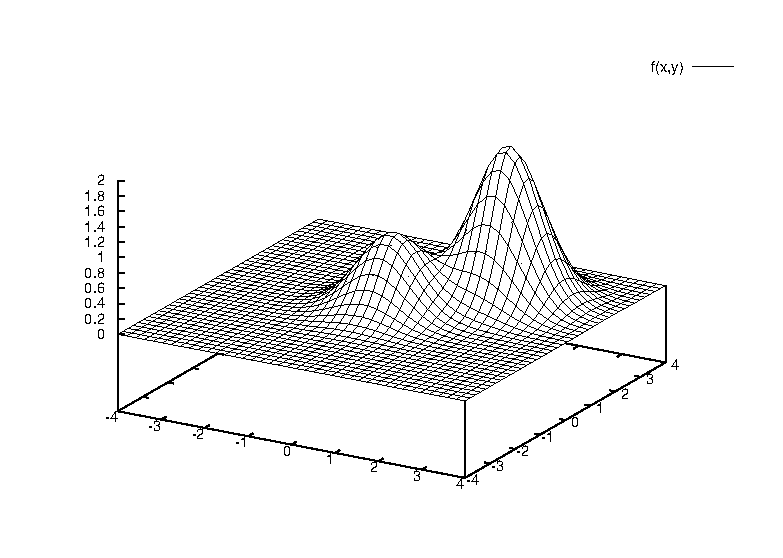
\includegraphics[scale=1]{Figures/mono.eps}
      \caption{An example of a difficult hill to climb.}
      \label{greedy}
    \end{figure} 
    If we imagine a climber to starting on the slope of the smaller of the two hills in figure \ref{greedy},
    we can see that once
    the climber reaches the summit of the smaller hill, it will assume that it has made it to the global
    maximum and exit.

    The advantage of greedy algorithms is that they're extremely fast, can sometimes get very close to what
    we want (and in some cases,
    \emph{exactly} what we want) and can be modified very easily. Simulated Annealing \cite{simAnneal} is a
    heuristically modified greedy algorithm that allows for `downhill' movement in an attempt to negate termination
    at local maxima and many others exist too. The pool of greedy algorithmic solutions is a rich environment
    from which to draw candidate algorithms that will fit my criteria.

    \subsection{The base algorithm} 
      In 2008 -- during my $2^{nd}$ year of university\footnote{This was a self guided research project with no
      overriding goal (other than to solve the problem as best I can). It is responsible for my current interest
      in the topic of computational complexity.} -- I wrote a greedy deterministic
      algorithm with the aim to solve the vertex cover problem.

      I met -- as you can imagine -- with limited success, but I did develop this main algorithm which greedily
      produces a cover which can be considered `reasonably' accurate.  
     
      The algorithm at its simplest, consists of a set of heuristics which are applied to the two vertices at
      either end of each edge. We define the terms \emph{used}/\emph{marked} as synonyms for a vertex being a
      member of the covering set or for an edge being connected to a member of the covering set. We also define
      the term \emph{visited} to indicate whether a vertex has already been considered by the algorithm or not.
      The main covering routine of the program is outlined in figure \ref{baseAlgo}.

      \begin{figure}
      \begin{itemize*}
        \item [] \textbf{Vertex\_Cover(Graph $G(V,E)$)}
        \begin{enumerate*}
          \item For each $e \in E$, and $v_1, v_2 \in V \mid v_1 = fst(e) \land v_2 = snd(e)$ 
          \begin{enumerate*}
            \item If neither $v_1$ or $v_2$ is visited\ldots 
            \begin{itemize*}
              \item [] Mark the vertex with the highest number of adjacent unmarked edges. In the event
                       of a tie -- mark $v_1$.
            \end{itemize*} 
            \item Else If either vertex has been marked\ldots  
            \begin{itemize*}
              \item [] Do nothing.
            \end{itemize*}
            \item Else If neither vertex has been marked\ldots  
            \begin{itemize*}
              \item [] If one vertex has been visited, but the other one hasn't. Mark the one
                       with the most adjacent unmarked edges. In the event
                       of a tie -- mark $v_1$.
            \end{itemize*}
            \item Else if both vertices are visited and unmarked\ldots  
            \begin{itemize*}
              \item [] If neither vertex has been marked, mark the one with the highest
                       number of adjacent edges. In the event of a tie, do nothing
            \end{itemize*}
          \end{enumerate*}
        \end{enumerate*}
      \end{itemize*}
      \caption{The basic greedy algorithm for vertex covering.}
      \label{baseAlgo}
      \end{figure}
      These rules as they are work well for graphs with a trivial topology and can exactly solve many handmade
      graphs. It does, however, fall down when a topologically complicated graph is presented to it.


    \subsection{Some improvements}

      Lets imagine a graph hub $h$ (a single vertex with a very high degree) and then picture every edge emerging from it
      connecting to hubs $x_0 \ldots x_n$ that have a smaller degree. The base algorithm will likely cover $h$ and
      then go on to cover all of $x_0 \ldots x_n$. I don't know of a way to prevent this from happening
      during the covering process,
      but post-processing the graph to uncover those vertices that are completely surrounded by covered ones is certainly
      achievable (figure \ref{fig:uncover}).
  
      \begin{figure}
      \begin{itemize*}
        \item [] \textbf{Optimise\_Cover(Graph $G(V,E)$)}     
        \begin{enumerate*}
          \item For each marked vertex $v \in V$
          \begin{enumerate*}
            \item If $v$ is totally surrounded by marked vertices\ldots
            \begin{itemize*}
              \item [] Unmark $v$
            \end{itemize*}
          \end{enumerate*}
        \end{enumerate*}
      \end{itemize*}
      \caption{How the post-processing algorithm executes.}
      \label{fig:uncover}
      \end{figure} 


      The greatest problem for any greedy algorithm that acts upon graphs though, is the way it traverses
      them. There are various heuristics that can be used to guide the traversal of a graph.
      We can order the graph such that each edge is connected to preceding one as a kind of `tree' structure
      in an attempt to `cascade' a greedy vertex cover throughout the graph. 

      One of the most obvious methods for guiding the traversal of the graph is to impose max-min
      ordering on the vertices. 
      Lets consider an example of this, the vertices in the covering set are bolded green:
      \begin{figure}[ht]
        \begin{minipage}[b]{0.5\linewidth}
          \centering
          \includegraphics[scale=0.5]{Figures/wrong.eps}
          \caption{How the algorithm may cover a graph like this.}
          \label{fig:graph1}
        \end{minipage}
        \hspace{0.5cm}
        \begin{minipage}[b]{0.5\linewidth}
          \centering
          \includegraphics[scale=0.5]{Figures/right.eps}
          \caption{How the algorithm \emph{should} cover a graph like this.}
          \label{fig:graph2}
        \end{minipage}
      \end{figure}

      In the left example, the set $VC_l= \{1,3,5,7,10,11\}$ which is sub-optimal when compared to
      $VC_r = \{2,4,6,8,9\}$. Against all our intuition, covering the vertex with the highest degree actually
      results in a sub-optimal conclusion!

      So it appears that imposing a max-min degree ordering on the vertices is not really a viable solution
      -- at least not on its own.

      A possible combination we could have is combining the degree of a vertex with its cluster coefficient.
      We can formulate a heuristic as follows, we impose our max-min ordering as before and define a $y : 0 < y < 1$
      as a coefficient discriminant. This would be set at a sufficiently high level (say two std. deviations above the
      mean) so that only hubs that are highly clustered are covered.

      The rationale for this is that each cluster has to have at least two of its vertices covered. So we may as
      well at least cover the vertex that has the highest degree and cluster coefficient. I realise that this
      can fall into the `intuition trap' above, but preparing for every eventuality is infeasible.

    \subsubsection{Resulting algorithms}

      We now have a set of three `modules'\footnote{There are many, many more which can be used also. This is a very
      restricted set due to the time constraints and other avenues of investigation.}
      that can be used and combined to produce greedy algorithms. There is the
      base rules, the vertex removal post-processing and the ordering-and-covering pre-processing methods. With
      these in mind, I have produced 4 algorithms for testing and comparison:

      \begin{enumerate*}
        \item The base algorithm only -- no pre- or post-processing.
        \item Base with post-processing.
        \item Base with pre-processing.
        \item Base with both pre and post-processing
      \end{enumerate*} 
      We expect the speed of the first algorithm to be the highest as it is just applying the heuristics (as every
      algorithm will do) with no special processing. The accuracy of the first algorithm is expected to be the
      lowest of the four though. Conversely, we expect high accuracy and low speed from algorithm four.

    \subsection{Testing and analysis}
      The four algorithms were tested on the two separate sets, recording both the times and resulting covers.
      The first set consisted of graphs generated by my own graph generation model and the second set
      contained graphs constructed by model RB with hidden optimal values for the vertex cover.
  
      \subsubsection{First set}
        The first set was eight graphs that were produced by my graph generation method (section \ref{sec:tgf}). 
        Below is the list of Graphs 1--8 with information about them. Following that is tables of the results
        of each algorithm running on each graph. Table \ref{table:res1} displays the returned value of the
        algorithms, whilst table \ref{table:res12} applies equation \ref{eq:conversion} to convert these
        numbers into percentages of coverage.

        All runs were performed three times and a mean running time was obtained, these times were plotted
        on the charts in section \ref{sec:aggRes}.

        \begin{enumerate*}
          \item $|V| = 150,\quad|E|= 3632$, 30 cliques, MVC = 200
          \item $|V| = 225,\quad|E|= 7150$, 25 cliques, MVC = 200
          \item $|V| = 276,\quad|E|= 4041$, 69 cliques, MVC = 207
          \item $|V| = 280,\quad|E|= 8653$, 28  cliques, MVC = 252
          \item $|V| = 429,\quad|E|= 11837$, 39 cliques, MVC = 390
          \item $|V| = 966,\quad|E|= 57532$, 46 cliques, MVC = 920
          \item $|V| = 1140,\quad|E|= 59851$, 60  cliques MVC = 1080 
          \item $|V| = 1311,\quad|E|= 115019$, 69  cliques, MVC = 1242
        \end{enumerate*}

        \begin{table}[H]
          \begin{tabular}{| c | c | c | c | c | c | c | c | c |}
            \hline
                   &  Graph 1 & Graph 2 & Graph 3 & Graph 4 & Graph 5 & Graph 6 & Graph 7 & Graph 8  \\ \hline
            Algo 1 &  121     & 210     &  218    &  261    &  407    &  940    & 1104    &  1288    \\ \hline
            Algo 2 &  120     & 204     &  208    &  263    &  403    &  933    & 1096    &  1272    \\ \hline
            Algo 3 &  121     & 210     &  217    &  265    &  406    &  940    & 1105    &  1286    \\ \hline
            Algo 4 &  120     & 204     &  208    &  263    &  403    &  933    & 1096    &  1272    \\ \hline
    \textbf{Ideal}&\textbf{120}&\textbf{200}&\textbf{207}&\textbf{252}&\textbf{390}&\textbf{920}&\textbf{1080}&\textbf{1242}  \\ \hline
          \end{tabular}
          \caption{Results of the algorithms being run on the graphs of set 1.}
          \label{table:res1}
        \end{table}

        \begin{table}[H]
          \begin{tabular}{| c | c | c | c | c | c | c | c | c |}
            \hline
                   &  Graph 1        & Graph 2      & Graph 3         & Graph 4         & Graph 5         & Graph 6         & Graph 7         & Graph 8         \\ \hline
            Algo 1 &100.83\%         &105\%         &105.31\%         &\textbf{103.57\%}&104.35\%         & 102.17\%        & 102.22\%        & 103.70\%        \\ \hline
            Algo 2 &\textbf{100\%}   &\textbf{102\%}&\textbf{100.48\%}&104.36\%         &\textbf{103.33\%}&\textbf{101.41\%}&\textbf{101.48\%}&\textbf{102.41\%}\\ \hline
            Algo 3 &100.83\%         &105\%         &104.83\%         &105.15\%         &104.10\%         & 102.17\%        & 102.31\%        & 103.54\%        \\ \hline
            Algo 4 &\textbf{100\%}   &\textbf{102\%}&\textbf{100.48\%}&104.36\%         &\textbf{103.33\%}&\textbf{101.41\%}&\textbf{101.48\%}&\textbf{102.41\%}\\ \hline
          \end{tabular}
          \caption{Coverages of each of the algorithms run on the graphs of set 1. Best are bolded.}
          \label{table:res12}
        \end{table}



      \subsubsection{Second set}
         
        The second set of algorithms also consisted of eight graphs, drawn from the benchmarks at
        \url{http://www.nlsde.buaa.edu.cn/~kexu/benchmarks/graph-benchmarks.htm}. These graphs have the
        following attributes.

        \begin{enumerate*} 
          \item $|V| = 595,\quad|E|= 28143$, 35 cliques, MVC = 560
          \item $|V| = 760,\quad|E|= 41605$, 40 cliques, MVC = 720
          \item $|V| = 900,\quad|E|= 58579$, 45 cliques, MVC = 900
          \item $|V| = 1100,\quad|E|= 80035$, 50  cliques, MVC = 1100
          \item $|V| = 1219,\quad|E|= 94226$, 53 cliques, MVC = 1219
          \item $|V| = 1344,\quad|E|= 109601$, 56 cliques MVC, = 1344
          \item $|V| = 1475,\quad|E|= 125982$, 59 cliques MVC, = 1475
          \item $|V| = 3900,\quad|E|= 572774$, 100 cliques, MVC = 3900
        \end{enumerate*} 

        
       
        \begin{table}[H]
          \begin{tabular}{| c | c | c | c | c | c | c | c | c |}
            \hline
                   &  Graph 1 & Graph 2 & Graph 3 & Graph 4 & Graph 5 & Graph 6 & Graph 7 & Graph 8  \\ \hline
            Algo 1 &  569     & 729     & 912     & 1114    & 1234    & 1360    & 1492    & 3934     \\ \hline
            Algo 2 &  567     & 728     & 912     & 1112    & 1230    & 1359    & 1492    & 3930     \\ \hline
            Algo 3 &  569     & 729     & 912     & 1114    & 1234    & 1360    & 1492    & 3928     \\ \hline
            Algo 4 &  567     & 728     & 910     & 1112    & 1230    & 1359    & 1488    & 3926     \\ \hline
    \textbf{Ideal}&\textbf{560}&\textbf{720}&\textbf{900}&\textbf{1100}&\textbf{1219}&\textbf{1344}&\textbf{1475}&\textbf{3900}  \\ \hline
          \end{tabular}
          \caption{Results of the algorithms being run on the graphs of set 2.}
          \label{table:res2}
        \end{table}

        \begin{table}[H]
          \begin{tabular}{| c | c | c | c | c | c | c | c | c |}
            \hline
                   &Graph 1          & Graph 2         & Graph 3         & Graph 4         & Graph 5        & Graph 6         & Graph 7         & Graph 8         \\ \hline
            Algo 1 &101.6\%          &101.25\%         &101.33\%         & 101.27\%        & 101.23\%       & 101.19\%        &101.15\%         &100.87\%         \\ \hline
            Algo 2 &\textbf{101.25\%}&\textbf{101.11\%}&101.33\%         &\textbf{101.09\%}&\textbf{100.9\%}&\textbf{100.89\%}&101.15\%         &100.76\%         \\ \hline
            Algo 3 &101.6            &101.25\%         &101.33\%         & 101.27\%        & 101.23\%       &101.19\%         &101.15\%         &100.71\%         \\ \hline
            Algo 4 &\textbf{101.25\%}&\textbf{101.11\%}&\textbf{101.11\%}&\textbf{101.09\%}&\textbf{100.9\%}&\textbf{100.89\%}&\textbf{100.88\%}&\textbf{100.66\%}\\ \hline
          \end{tabular}
          \caption{The coverage of each algorithm on each graph in set 2. Best are bolded.}
        \end{table}
   
      \subsection{Aggregate results} \label{sec:aggRes}
        Viewing the results above, we can see that the hiding of optimal solutions doesn't
        particularly impact the solvability of an instance. Over both sets, the returned cover is usually
        about 0-15 vertices over the optimal.
  
        In terms of comparative performance, algorithm 4 performed as well as was expected with algorithm
        1 doing worst out of the four -- with the exception of graph 4 in set 1, where algorithm 4 clearly
        outperformed the other algorithms. The accuracies of the algorithms are plotted in figure 
        \ref{fig:greedyResults} and this indicates -- with some exceptions in set 2 -- that the 
        post-processing of algorithm is responsible for the accuracies being close to 100\% 
   
        This shows us that the modules we were adding to the main graph covering routine were working as
        intended, each one gradually improving the returned result in general. It is interesting to note that each
        of these random examples have approximated a cover within a factor 1.3606\ldots. If it can be shown that 
        these algorithms are a \emph{constant-factor approximation algorithm} for a constant $c < 1.3606\ldots$
        P = NP is implied. This will be expanded upon in the conclusions and further work sections (\ref{sec:results}). 

        
        \begin{figure}[H] 
          \begin{minipage}[b]{0.5\linewidth}
            \centering
            \includegraphics[scale=0.7]{Figures/plot1Res.eps}
          \end{minipage}
          \hspace{0.8cm}
          \begin{minipage}[b]{0.5\linewidth}
            \centering
            \includegraphics[scale=0.7]{Figures/plot2Res.eps}
          \end{minipage}
          \caption{The coverages of the algorithms on both sets. Lower is better.}
          \label{fig:greedyResults} 
        \end{figure}


        \begin{figure}[H]
          \begin{minipage}[b]{0.5\linewidth}
            \includegraphics[scale=0.7]{Figures/plot1Time.eps}
          \end{minipage}
          \hspace{0.8cm}
          \begin{minipage}[b]{0.5\linewidth}
            \centering
            \includegraphics[scale=0.7]{Figures/plot2Time.eps}
          \end{minipage}
          \caption{Time taken in seconds for the algorithms over both sets.}
          \label{fig:greedyTimes}
        \end{figure}
  

      In the time comparison graphs above, we can see that the algorithms are roughly equal in terms
      of running time in seconds. The reason for this is because of the asymptotic dominance that the
      base algorithm has which will be explained in the next section.
       

      \subsection{Asymptotic time analysis}
        Because the fourth algorithm produced contains all of the modules, it makes sense to analyse this
        algorithm and compute a Big-O upper bound on the running time. For this, we define $v := |V|, e := |E|$.
        Due to the design of the graph structure, directly accessing vertices and edges by id is $O(1)$. 

        \subsubsection{Base algorithm}
          The base algorithm consists of a top level loop that iterates over the members of $E$ ($L_0$), this will
          take $e$ time. Inside the loop, there are five upper level if statements ($IF_0 \ldots IF_4$). In
          practice -- because we are interested in the wort case running time -- we shall only analyse the
          If statement that takes the longest. This turns out to be $IF_2$ which contains another four if
          statements $IF_{20} \ldots IF_{23}$, of which $IF_{23}$ has $IF_{230}$
          and $IF_{231}$ which are nearly identical.
          See figure \ref{fig:asyBase} for a structured listing of the least optimal execution path.  
           
          \begin{figure}[H]
            \begin{itemize*}
              \item [] For all $e \in E$ -- $\mathbf{L_0}$
              \item [] Assign $v_1$ and $v_2$ to the values of the vertex ids in $e$ -- $\mathbf{VA_0}$, $\mathbf{VA_1}$
              \item [] Assign $vm_1$ and $vm_2$ to the number of unmarked edges for $v_1$ and $v_2$
                       respectively -- $\mathbf{VME_0}$, $\mathbf{VME_1}$ 
              \begin{itemize*}
                \item [] \ldots( CODE REMOVED )\ldots
                \item [] If neither vertex has been marked -- $\mathbf{IF_2}$
                \begin{itemize*}
                  \item [] \ldots( CODE REMOVED )\ldots 
                  \item [] If neither vertex has been visited -- $\mathbf{IF_{23}}$
                  \begin{itemize*}
                    \item [] If (comparison of marked edges) -- $\mathbf{IF_{230/1}}$ 
                    \item [] \hspace{20mm}then mark one ($\mathbf{MV_0}$) and visit both ($\mathbf{VV_0}$, $\mathbf{VV_1}$).  
                  \end{itemize*} 
                \end{itemize*} 
                \item [] \ldots( CODE REMOVED )\ldots
              \end{itemize*}
            \end{itemize*}
            \caption{Brief top level view of the longest execution path within the algorithm.
                     The bottom level result of all the if statements are the same: (a vertex get marked and
                     zero or more get visited).}
            \label{fig:asyBase}         
          \end{figure}   

          Referring back to section \ref{sec:asyGraph} we see that the values for $MV_x$, $VME_x$,
          $VA_x$ and $VV_x$ are
          $O(v-1)$, $O(v-1)$, $O(1)$ and $O(1)$ respectively. Asymptotic convention lists binary comparisons as being
          $O(1)$ time complexity, so we will insert $9O(1)$ for the nine if comparisons.  

          Assuming that the algorithm will follow this path for every
          iteration of the loop $e$, we can see that the worst case running time is:
          \begin{align*}
          Cover(G) &\in  e \times (2O(1) + 2O(v-1) + O(v-1) + 2O(1) + 9O(1)) \\
                   &\in e \times(O(3v-3) + O(12)) \\
                   &\in O(3ve - 3e + 12e) \\
                   &\in O(ve)  
          \end{align*}
          As is customary in infinite asymptotics, we keep only the values that grow the fastest as the variables
          in the function increase to infinity. 

          After this function $Cover(G)$ is executed, a supplementary validator $ValidCover(G)$ runs. All it
          does is check that each edge is connected to at least one marked vertex. This, predictably
          makes the time complexity $ \in O(e)$.
          
        \subsubsection{Preprocessing algorithm}
          The pre-processing algorithm works out the mean degrees and cluster coefficients of the vertices.
          Once it has these it calculates
          the standard deviation of both the degrees and cluster coefficients in the graph.

          It then iterates through all of the vertices and marks
          all those with a degree that is greater than equal to two standard deviations above the mean and with a
          cluster coefficient that is greater than or equal to one standard deviation above the mean.

          This iterates over the entirety of the list, but only sequentially, so we have $PreProc(G) \in O(v + v + v + v)$
          which is just $PreProc(G) \in O(v)$ 

        \subsubsection{Post-processing algorithm}  
          Post processing involves checking that every vertex that is marked is surrounded by marked vertices.
          In the worst case, every vertex is connected to every other one. This algorithm has two nested loops,
          one that loops over each $i \in V$ with an inner loop going over $V \setminus \{i\}$.  

          This presents the most interesting example of time complexity so far. The program makes $v(v-1)$
          comparisons, we multiply out and truncate the trailing $v$ term. This results in 
          $PostProc(G) \in O(v^2)$. 

        \subsubsection{Putting it all together}
         
          We now have time complexities for the modules and can add them together if we care to. However, 
          due to Big-O notation displaying only the largest growth factor of a function, every algorithm
          has an upper bound time complexity of $O(ve)$. We can prove this by observing that:
          \begin{equation}
             \lim_{v,e \to \infty} v^2 - ve = -x
          \end{equation}       
          where $x \in \mathbb{N}$ and $e >> v$ since there are typically a lot more edges than vertices
          in any given graph.
         
          In conclusion, the upper bound time complexity for the greedy algorithms is $O(ve)$ where $v = |V|$
          and $e = |E|$.
    

%%%%%%%%%%%%%%%%%%%%%%%%%%%%%%%%%%%%%%%%%%%%%%%%%%%%%%%%%%%%%%%%%%%%%%%%%%%%%%%%%%%%%%%%%%%%%%%%%%%%%%%%%%%%%%%%%%%%%%%
%  --------------------------------------------  NEURAL NETWORKS -------------------------------------------------
%%%%%%%%%%%%%%%%%%%%%%%%%%%%%%%%%%%%%%%%%%%%%%%%%%%%%%%%%%%%%%%%%%%%%%%%%%%%%%%%%%%%%%%%%%%%%%%%%%%%%%%%%%%%%%%%%%%%%%%

  \section{Artificial neural networks} \label{sec:ANN}
    \begin{center}
      \emph{Where the topic of artificial neural networks is explored. The difficulties explained, results
           produced and analyses performed.}
    \end{center}
    For this part of the experiment, I implemented a framework to build and train artificial neural networks (ANNs).
    This framework allows a user to build an acyclic feedforward ANN of arbitrary size and makes
    use of an implementation of the backpropagation algorithm to train the network.

    The actual framework itself
    is incomplete, as only the functionality that I required was implemented. A possible future project could be
    to extend this loose collection of classes and expand them into a more functional library.
    If you are unfamiliar with the workings of ANNs, please refer to appendix \ref{primer}.

    ANNs were selected over other machine learning methods due to their resistance to potentially 
    noisy data, high processing speed and relative simplicity in comparison to more complicated
    techniques like Bayesian belief networks -- which may have been more suitable due to the uncertainty
    surrounding which features indicate whether vertices belong in the covering set or not.


    \subsection{Framework architecture}
      The ANN contains 2 classes at the top level, the CompUnit class which is a catch-all class for the many different
      types of computation unit that the networks could employ and the ANN class itself which handles network evaluation
      and training functions as well as saving and loading from file.

      The other classes directly inherit from and override the CompUnit class, these are PerceptUnit, BasicSigUnit,
      ClassSigUnit and TanhUnit.
      The only real difference between these classes is in the activation and error functions:
 
      \begin{itemize*}
        \item \textbf{PerceptUnit} - - This unit just outputs an unthresholded combination of its outputs. It 
                                       also uses ordinary linear error calculation $(t_k - o_k)$. It is
                                       suitable for networks that attempt to fit linear data.
        \item \textbf{BasicSigUnit} -- This unit applies the sigmoidal function \begin{equation} \label{SigFunc} 
                                       \sigma(y) = \frac{1}{1+e^{-y}} \end{equation} to the input and outputs
                                       the result. This function is continuous and outputs a value from
                                       -1 to 1. This is ideal for the hidden units of the network. The
                                       error function is the shown in the example above. 
        \item \textbf{ClassSigUnit} -- The activation function for this unit is the same as above, the difference
                                       lying in the error term function. This unit is specifically designed to 
                                       differentiate between classes as according to the two class \emph{cross entropy} 
                                       section \ref{sec:crosse}
                                       of the network. This means that a probability is returned -- 
                                       0 for class 0 and 1 for class 1 --
                                       rather than an absolute value as a BasicSigUnit would. This value is then subject
                                       to a discriminant $y =0.5$ to sort the input vector into one of the classes. 
        \item \textbf{TanhUnit} --  The TanhUnit class has $f(x) = \tanh(x)$ as the activation function.
                                    The tanh function is actually related to
                                    the sigmoidal by the equation:
                                    \begin{equation}
                                      2\sigma(x) = 1 + \tanh\left (\frac{x}{2} \right )
                                    \end{equation}
                                    It is not actually used in any of the trained networks and was included
                                    while testing.
       \end{itemize*} 

      The ANN instances that were to be trained in the dissertation only utilise the BasicSigUnit
      and the ClassSigUnit units.  
      There are also a number of conventions that the ANN framework uses to keep things in order:
      \begin{itemize*}
        \item All units (excluding those in the input layer) have a constant input of 1.
              This input does have a random weight like all
              the other inputs however. By convention, this input comes from a unit with an id of $-1$.
        \item All of the inputs into the network are units with no input list and a flag that
              indicates they are part of the input layer.
        \item All of the units in the output layer have no output list and a flag that indicates that
              they are in the output layer.
      \end{itemize*}
   

      \subsubsection{Calculations and training functions}

        A calculation requires a set of input units and the corresponding values for each.
        In practice, this is modelled by a 2-dimensional array. The ANN class prepares each unit
        by giving it the input values it needs and then invokes the units fire() method. The
        unit then calculates its output value and returns the output along with a list of the
        units that the output is to go to.

        The ANN uses this information to prepare and fire the other units in the network and
        continues to operate in this manner until all of the units have fired. The output from
        the network is collected and returned. For training, the output is used in conjunction with
        the backpropagation algorithm as detailed in appendix \ref{backprop}
          
        To train the network using the graph instances created by the test case generator, it was
        decided that the network would be given features of individual vertices and then it would output
        the probability of the vertex being in the covering set.
        Backpropagation would then ensue, applying the correct result to the network and adjusting the weights.          

        Validation is done through a separate instance set. After every 5 training epochs, the ANN is run over 
        these instances, and the percentage of misclassified examples is worked out. If the error percentage is
        under a thresholded amount of 10\% then the training of the ANN is terminated.
           
        As a choice of training function, I chose backpropagation. Unfortunately, this has a propensity to
        converge to a target function slowly. Backpropagation is the easiest of all the training functions
        to understand, implement and tweak, but it has been widely shown to be far too slow for practical
        training purposes. \cite{Fahlman88anempirical}\cite{Cascade-correlation}In this dissertation,
        I also found it to be too slow, but did
        not have enough time to change the learning function to something more suitable. 
    
        If I were given the chance to do the dissertation again, I would choose a better learning function,
        such as cascade correlation \cite{Cascade-correlation} or maybe even a quick propagation variant. 

     \subsection{ANN instance design}

       \subsubsection{Feature selection}

         Feature selection was largely a case of thinking of a number of vertex properties and selecting those which
         would likely help in determining whether a particular vertex was part of the covering set or not. These
         features were used to create a number of exhaustive data sets (the details of which are explained in
         section \ref{sec:stats}).

         Each instance in each set was then analysed by an implementation of n\'{a}ive Bayes which trained itself on 80\%
         of the records and attempted to correctly classify the remaining 20\%.
  
         The n\'{a}ive Bayes algorithm returns an accuracy percentage of how well it classified the remaining examples
         in each instance. This data was then collated to produce plottings (said plottings can also be found in
         appendix \ref{app:DS}) which gave me a visual representation of how good of an indicator the features
         were.

         In the end the selected features were:
         \begin{itemize*}
           \item vertex degree / maximum possible indegree.
           \item cluster coefficient of the vertex.
           \item mean (vertex degree / maximum possible indegree) of all the neighbouring vertices.
           \item mean cluster coefficient of all the neighbours.
           \item percentage of adjacent vertices covered. 
         \end{itemize*}      
  
         The selection of the last feature was a controversial one and, in hindsight, was not the 
         best feature I could have selected. The reasons for this is that the training instances
         are already optimally covered and each vertex in the graph will have a nonzero figure for
         this attribute.

         A graph that has to be covered though, will initially have zero figures for this feature
         at each vertex -- since there is no covered vertices in the graph, 
         which means that the feature is ill-representative of the covering process.

         Another problem is that its inclusion actually makes the problem linearly separable for
         connected graphs. This can be seen if we consider that a vertex that is not in the vertex
         cover will be surrounded totally by covered vertices so the adjacent covered vertices feature
         will be 1. Whereas, a vertex that is in the cover will be adjacent to at least one uncovered
         vertex, making the adjacent covered vertices feature a figure $< 1$.  
         
       \subsubsection{Instance topology}
         The instances to be trained were 5,5,5,1 neural networks. Figure \ref{fig:anns} shows the
         topology of the network. `S' units are BasicSigUnits while the `C' on unit 15 is a
         ClassSigUnit.
         
         \begin{figure}
           \centering
           \includegraphics[scale=0.75]{Figures/annFig.ps}
           \caption{The structure of the ANN. Not shown is the bias input to each unit from unit -1.}
           \label{fig:anns}
         \end{figure}  

         This topology works well for the lower training sets (where $0.2 \leq \alpha \leq 0.4$), but
         doesn't work so well for the training sets where $\alpha$ is larger (sets $ 0.5 \leq \alpha \leq 0.9$).
         Adding more units or hidden layers to the networks acting on the larger sets didn't appear to
         improve convergence or accuracy performance. 

     \subsection{Training} \label{sec:ANNTrain}
       Originally I created eight neural networks, using one for each data set. After training these in parallel
       on different machines, I observed that the training time taken for the larger sets was well in excess of
       what I had expected. Eventually, I terminated the training and tried a different approach.

       Instead of using separate networks, I used one that was sequentially trained on the data sets.
       Again, the training proceeded well up to $\alpha = 0.5$ where convergence was slowed down to a near stop.
       After training on $\alpha = 0.5$ for 2 whole weeks with 100\% uptime, the training effort was again
       aborted at epoch 7255 with an absolute error (the number of misclassified vertices) percentage of
       12.23\%.

       \begin{figure}
         \centering
         \includegraphics{Figures/Training5.eps}
         \caption{The network was trained to Epoch 7255 before it was forcibly terminated.}
         \label{fig:5Training}
       \end{figure}

       As shown in figure \ref{fig:5Training}, the function was still converging, albeit
       in a meandering fashion. If given more time, it may eventually converge to a minimum, but significantly
       more time would need to be allocated to the training phase for it to happen. The network may then be trained
       on the sets where $\alpha > 0.5$, but I suspect that they will converge much slower if they even converge
       at all.      

       Whenever a training set was completed, the new network was tested on its own validation set, but also
       was regression tested on all of the validation sets of the previous training examples.
       Out of curiosity, I also tested the networks against the validation sets of successive training examples to 
       see how they fared. Table \ref{table:absErr} shows the absolute error of the neural networks being
       trained up to a certain set and then being validated against all sets.

       \begin{table}[H]
         \centering
         \begin{tabular}{|c|c|c|c|c|c|}
           \hline
           &\multicolumn{5}{|c|}{Trained up to set} \\
           \cline{2-6}
           &  & 0.2 & 0.3 & 0.4 & 0.5 \\ \cline{2-6}
           \multirow{4}{*}{Tested on set}
           & 0.2 & \textbf{6}     & 0    & 0    & 0  \\ \cline{2-6}
           & 0.3 & 1255  &\textbf{51}    &16    & 1118 \\ \cline{2-6}
           & 0.4 & 3445  &2160  &\textbf{511}   & 939 \\ \cline{2-6}
           & 0.5 & 11465 &16266 &3111  & \textbf{1978} \\ \cline{2-6}
           & 0.6 & 48200 &58346 &37130 & 8882 \\ \cline{2-6}
           & 0.7 & 91866 &95752 &92523 & 34278 \\ \cline{2-6}
           & 0.8 & 141283&146981&144203&88651 \\ \cline{2-6}
           & 0.9 & 167781&175560&172887&168426\\
           \hline
         \end{tabular}
         \caption{The absolute error of testing trained networks.}
         \label{table:absErr}
       \end{table}
  
       We can observe a clear diagonal of relatively low absolute error at each coordinate $[n,n]$.
       This is what we hoped for and -- as an added bonus -- we can see that as the training has proceeded,
       the network mostly retains its knowledge on how to solve instances from the previous training sets.

     \subsection{Running the network}
       Two methods of using the ANNs to obtain a vertex were employed: vertex-wise and edge-wise processing.
       First the given ANN and graph files were parsed and their objects constructed, then -- for the
       vertex-wise processing -- the graph is traversed over the set of all vertices, with each one having its
       essential information parsed and inputted to the network. The program covers the vertex if the returned
       value is $\geq 0.5$.
       
       Once this is done, the integrity of the cover is verified by processing the graph by edge, which is exactly how
       the greedy algorithms verify their covers. If a violating edge is detected, the algorithm processes it
       in the same manner as the edge-wise algorithm does.

       The edge-wise processing compares the network return values of both vertices and covers the one that has
       been determined to be most likely a member of the covering set.

       \subsubsection{Vertex-wise processing results}

         Below are two tables of results, one for each set that was processed by the vertex-wise system.
         The ANN used in each test was the same, but with different level of training. 

         \begin{table}[H]
           \begin{tabular}{| c | c | c | c | c | c | c | c | c |}
             \hline
                     &  Graph 1 & Graph 2 & Graph 3 & Graph 4 & Graph 5 & Graph 6 & Graph 7 & Graph 8  \\ \hline
             ANN 0.2 &  145     & 219     & 257     & 273    & 414    & 956    & 1119    & 1291     \\ \hline
             ANN 0.3 &  145     & 221     & 262     & 274    & 419    & 953    & 1124    & 1297     \\ \hline
             ANN 0.4 &  143     & 222     & 264     & 274    & 419    & 956    & 1125    & 1300     \\ \hline
             ANN 0.5 &  143     & 223     & 264     & 274    & 419    & 956    & 1125    & 1299     \\ \hline
      \textbf{Ideal}&\textbf{120}&\textbf{200}&\textbf{207}&\textbf{252}&\textbf{390}&\textbf{920}&\textbf{1080}&\textbf{1242}  \\ \hline
           \end{tabular}
           \caption{Cover results for set 1 using vertex-wise processing.}
           \label{table:res1Vert}
         \end{table}

         \begin{table}[H]
          \begin{tabular}{| c | c | c | c | c | c | c | c | c |}
            \hline
                   &  Graph 1 & Graph 2 & Graph 3 & Graph 4 & Graph 5 & Graph 6 & Graph 7 & Graph 8  \\ \hline
            ANN 0.2 &  586     & 745     & 931     & 1136    & 1258    & 1385    & 1515    & 3968     \\ \hline
            ANN 0.3 &  588     & 747     & 936     & 1138    & 1260    & 1390    & 1521    & 3979     \\ \hline
            ANN 0.4 &  588     & 751     & 937     & 1139    & 1262    & 1391    & 1523    & 3982     \\ \hline
            ANN 0.5 &  588     & 752     & 937     & 1139    & 1263    & 1391    & 1523    & 3982     \\ \hline
    \textbf{Ideal}&\textbf{560}&\textbf{720}&\textbf{900}&\textbf{1100}&\textbf{1219}&\textbf{1344}&\textbf{1475}&\textbf{3900}  \\ \hline
          \end{tabular}
          \caption{Cover results for set 2 using vertex-wise processing.}
          \label{table:res2Vert}
        \end{table}

      \subsubsection{Edge-wise processing results}         
       
        \begin{table}[H]
          \begin{tabular}{| c | c | c | c | c | c | c | c | c |}
            \hline
                    &  Graph 1 & Graph 2 & Graph 3 & Graph 4 & Graph 5 & Graph 6 & Graph 7 & Graph 8  \\ \hline
            ANN 0.2 &  124     & 217     & 238     & 269    & 407    & 946    & 1110    & 1292     \\ \hline
            ANN 0.3 &  128     & 219     & 240     & 275    & 415    & 955    & 1125    & 1302     \\ \hline
            ANN 0.4 &  143     & 217     & 257     & 272    & 410    & 952    & 1120    & 1294     \\ \hline
            ANN 0.5 &  126     & 216     & 244     & 267    & 408    & 945    & 1109    & 1291     \\ \hline
     \textbf{Ideal}&\textbf{120}&\textbf{200}&\textbf{207}&\textbf{252}&\textbf{390}&\textbf{920}&\textbf{1080}&\textbf{1242}  \\ \hline
          \end{tabular}
          \caption{Cover results for set 1 using edge-wise processing.}
          \label{table:res1Edge}
        \end{table}

        \begin{table}[H]
         \begin{tabular}{| c | c | c | c | c | c | c | c | c |}
           \hline
                  &  Graph 1 & Graph 2 & Graph 3 & Graph 4 & Graph 5 & Graph 6 & Graph 7 & Graph 8  \\ \hline
           ANN 0.2 &  592     & 754     & 940     & 1148    & 1268    & 1398    & 1530    & 3995     \\ \hline
           ANN 0.3 &  594     & 756     & 944     & 1147    & 1270    & 1398    & 1531    & 3998     \\ \hline
           ANN 0.4 &  592     & 759     & 941     & 1149    & 1220    & 1399    & 1531    & 3995     \\ \hline
           ANN 0.5 &  591     & 752     & 939     & 1147    & 1267    & 1396    & 1528    & 3998     \\ \hline
   \textbf{Ideal}&\textbf{560}&\textbf{720}&\textbf{900}&\textbf{1100}&\textbf{1219}&\textbf{1344}&\textbf{1475}&\textbf{3900}  \\ \hline
         \end{tabular}
         \caption{Cover results for set 2 using edge-wise processing.}
         \label{table:res2Edge}
       \end{table}

       \subsubsection{Discussion and plots}
         The results here are better than I had expected. They are, however rather inconclusive due to how
         inconsistent they are. This inconsistency is especially true for the covers produced by the
         edge-wise processing -- there doesn't appear to be a correlation
         between the accuracy of the cover and the set that the ANN was trained up to. Figures 
         \ref{fig:coverPlotsVP} and \ref{fig:coverPlotsEP} show plots of the values of the vertex covers
         against the ideal values.

         These plots show evidence of the inconsistency, but also trends in the solutions. There is a definite
         trend in the coverages for set 1 where the more highly trained ANNs result in a higher overall coverage.
         But, in set 2, ANN 0.5 gets a lower overall coverage in general than the other, less trained ANNs.   

         \begin{figure}
           \begin{minipage}[b]{0.5\linewidth}
            \centering
             \includegraphics[scale=0.7]{Figures/vertProcPer1.eps}
           \end{minipage}
           \hspace{0.8cm}
           \begin{minipage}[b]{0.5\linewidth}
            \centering
             \includegraphics[scale=0.7]{Figures/vertProcPer2.eps}
           \end{minipage}
           \caption{Plots of cover against instance for the vertex-wise processing method.}
           \label{fig:coverPlotsVP} 
         \end{figure}

         \begin{figure} 
           \begin{minipage}[b]{0.5\linewidth}
            \centering
             \includegraphics[scale=0.7]{Figures/edgeProcPer1.eps}
           \end{minipage}
           \hspace{0.8cm}
           \begin{minipage}[b]{0.5\linewidth}
             \centering
             \includegraphics[scale=0.7]{Figures/edgeProcPer2.eps}
           \end{minipage}
           \caption{Plots of cover against instance for the edge-wise processing method.}
           \label{fig:coverPlotsEP} 
         \end{figure}

         There is also a time overhead with processing the graphs by edge. Because the ANN cover blindly
         compares the two vertices of each edge, irrespective if they have been examined before or even
         covered previously, the program ends up making $|E|$ comparisons.

         The only functions that the code performs is the extraction of relevant data for a given vertex.
         this means that the covering routine has a worst case runtime of $O(e \times EXTRACT)$
         where $e = |E|$ and $EXTRACT$ is the worst case time complexity of the function to extract
         pertinent data from a vertex.

         The running times for edge-wise processing of the graph for sets 1 and 2 is plotted in figure
         \ref{fig:rtANN} below.

         \begin{figure} 
           \begin{minipage}[b]{0.5\linewidth}
            \centering
             \includegraphics[scale=0.7]{Figures/annTimes1.eps}
           \end{minipage}
           \hspace{0.8cm}
           \begin{minipage}[b]{0.5\linewidth}
             \centering
             \includegraphics[scale=0.7]{Figures/annTimes2.eps}
           \end{minipage}
           \caption{Plots of time taken against instance for the edge-wise processing method.
                    This data was generated on a computer with 8 core i386 Intel Xeon processor
                    running CentOS 5.5.}
           \label{fig:rtANN} 
         \end{figure}

         These graphs show us running times that are remarkably similar to the run time graphs of
         the greedy algorithms. This lends more weight to the results of our asymptotic analysis of
         those greedy algorithms that stated our main runtime growth factor is the number of edges
         $|E|$
                
     \subsection{Asymptotic analysis}
       This time analysis will cover the time taken for both the edge-wise and vertex-wise processing
       methods. First though, we establish the time taken to ready the ANN with information extracted
       from a vertex.

       There is 5 pieces of information provided to the ANN for a calculation, this information is:
       \begin{itemize*}
         \item vertex degree / maximum possible indegree.
         \item cluster coefficient of the vertex.
         \item mean (vertex degree / maximum possible indegree) of all the neighbouring vertices.
         \item mean cluster coefficient of all the neighbours.
         \item percentage of adjacent vertices covered. 
       \end{itemize*}
       
       It is fairly easy to see that the majority of this information gathering is information retrieval
       from the graph. Assuming our worst-case graph, we will have to iterate through the array
       of adjacent edges -- $O(n-1)$ time, where $n = |V|$ -- 3 times.

       We define $u$ as the number of units in the ANN. Because the ANN is an acyclic feedforward network,
       a simple calculation takes $O(u)$ time. Overall the time to prepare the network with the inputs,
       fire it and collect the inputs takes $O((n-1) + u) = O(n)$ time. 
       
       \paragraph{Vertex-wise processing:}
         The vertex-wise processing method simply calls this information retrieval function for each
         vertex in the graph. To vertex-wise process a graph therefore, we require $O(n^2)$ time. 
         
  
       \paragraph{Edge-wise processing:}
         The edge-wise processing method compares two vertices irrespective of whether they have been
         considered before or not. This means, that for every edge $e$ in the graph, the function to
         collect the inputs and fire the ANN is called twice. This gives us a running time of
         $O(e(2n)) = O(en)$ where  $e >> n$. This follows the trend set by the base greedy algorithm
         where there are much more edges than vertices in the graph.  

     \subsection{Improvements}
       There was problems with this approach to solving the vertex cover. Given another chance at
       implementing this part of the project, I would do some things differently:
       \begin{enumerate*}
         \item Use a different training function -- something like cascade-correlation which can dynamically
               grow and prune the network as the training proceeds.
         \item Conduct more in depth investigation into combinations of vertex and graph properties.
         \item Construct a simple tool that would allow me to view how the training of the network
               had progressed from start to finish in order to understand why convergence 
               is slow/ has stopped. 
         \item Perform a proper literature review to identify likely areas of fruitful research.  
       \end{enumerate*}
       
       The main point there is number four. I was impetuous in beginning this part of the project and
       didn't consider taking my time, reading up on other forays into this area and learning from
       their successes and  mistakes before making some of my own. Papers such as \cite{NPanns}, 
       \cite{Peterson89anew} and \cite{Peterson88neuralnetworks} would have been useful to gain
       insights into techniques for designing ANNs for effective combinatorial optimisation.


%%%%%%%%%%%%%%%%%%%%%%%%%%%%%%%%%%%%%%%%%%%%%%%%%%%%%%%%%%%%%%%%%%%%%%%%%%%%%%%%%%%%%%%%%%%%%%%%%%%%%%%%%%%%%%%%%%%%%%% 
%%%%%%%%%%%%%%%%%%%%%%%%%%%%%%%%%%%%%%%%%%% HYBRIDISATION %%%%%%%%%%%%%%%%%%%%%%%%%%%%%%%%%%%%%%%%%%%%%%%%%%%%%%%%%%%%%
%%%%%%%%%%%%%%%%%%%%%%%%%%%%%%%%%%%%%%%%%%%%%%%%%%%%%%%%%%%%%%%%%%%%%%%%%%%%%%%%%%%%%%%%%%%%%%%%%%%%%%%%%%%%%%%%%%%%%%%
 
  \section{Hybridisation}
    \begin{center}
      \emph{Where a hybrid algorithm is defined, planned, tested and analysed.}
    \end{center}
    A hybrid algorithm blends the properties of two or more different problem solving methodologies in order
    to correct for their deficiencies, or capitalise on their good properties. These algorithms have been used 
    in constraint satisfaction problems with success \cite{Gallardo_solvingweighted}.

    In my base greedy algorithm (section \ref{sec:GREEDY}), arbitrary vertex marking is done in order to resolve ties
    where the algorithm doesn't know which vertex to cover. This can very probably result in the program taking
    a computation path that will produce a sub-optimal solution.

    Conversely, the ANN performs no actual checking of the state of the graph at any point, preferring to 
    blindly process the graph until termination. This very probably results in needlessly covered vertices,
    such as ones that are totally surrounded by covered vertices.   

    I shall create a hybrid algorithm from greedy algorithm 4 and the pool of ANNs. At tiebreak points in the
    program, the ANNs will be consulted on which vertex to cover. This will follow a majority vote system, with
    the vertex with the most votes for covering being selected. 

    \subsection{The algorithm}
      At four points in algorithm 4, a tie between two vertices is broken by either covering one of them
      arbitrarily or by ignoring them. In the hybrid, a majority vote system is in place with ANNs 0.2-0.4.
      This is in order to force the algorithm into a resolution.

      At a tie between two vertices, the majority vote function is called. This runs both vertices through
      each ANN sequentially. After both vertices have been run through an ANN, it `votes' for the vertex 
      with the highest return value. The vertex with the highest votes gets covered and the algorithm 
      continues.
     
    \subsection{Running} 
      
      The algorithm was run on both test sets as is customary and the results collated
      in tables \ref{table:Hybrid1} and \ref{table:Hybrid2}. It is encouraging to note that the hybrid algorithm
      produces significant gains over the pure ANN algorithms and can usually match -- if not surpass -- the
      best results of greedy algorithms. 

      A look at the percentage coverage of the greedy algorithms
      versus the hybrid in figure \ref{fig:coverPlotsHy} confirms this observation shows a clear improvement over
      the greedy algorithms.  

      \begin{table}[H]
        \begin{tabular}{| c | c | c | c | c | c | c | c | c |}
          \hline
                  &  Graph 1 & Graph 2 & Graph 3 & Graph 4 & Graph 5 & Graph 6 & Graph 7 & Graph 8  \\ \hline
          Hybrid  &  120     & 201     & 207     & 257    & 400    & 935    & 1095    & 1279     \\ \hline
      \textbf{Ideal}&\textbf{120}&\textbf{200}&\textbf{207}&\textbf{252}&\textbf{390}&\textbf{920}&\textbf{1080}&\textbf{1242}  \\ \hline
           \end{tabular}
        \caption{Results for the Hybrid algorithm being run on set 1.} 
        \label{table:Hybrid1}
      \end{table}
 
      \begin{table}[H]
        \begin{tabular}{| c | c | c | c | c | c | c | c | c |}
          \hline
                 &  Graph 1 & Graph 2 & Graph 3 & Graph 4 & Graph 5 & Graph 6 & Graph 7 & Graph 8  \\ \hline
          Hybrid &  570     & 728     & 910     & 1112    & 1232    & 1355    & 1490    & 3926     \\ \hline
   \textbf{Ideal}&\textbf{560}&\textbf{720}&\textbf{900}&\textbf{1100}&\textbf{1219}&\textbf{1344}&\textbf{1475}&\textbf{3900}  \\ \hline
       \end{tabular}
       \caption{Results for the Hybrid algorithm being run on set 2.}
       \label{table:Hybrid2}
     \end{table}


     \begin{figure}[H]
       \begin{minipage}[b]{0.5\textwidth}
         \centering
         \includegraphics[width=\textwidth]{Figures/Hybrid1.eps}
       \end{minipage}
       \hfill
       \begin{minipage}[b]{0.5\textwidth}
         \centering
         \includegraphics[width=\textwidth]{Figures/Hybrid2.eps}
       \end{minipage}
       \caption{Comparison plots of percentage coverages for all the greedy algorithms vs the hybrid.}
       \label{fig:coverPlotsHy} 
     \end{figure}

     
    \subsection{Asymptotic analysis}
      The asymptotic analysis of this algorithm rides on the back of the analyses for greedy algorithm 4
      and for the vertex-wise processing method.

      In general, the 3 ANNs are invoked only a certain number of times while processing the graph, lets call that
      number $c : 0 \leq c < e$. At that point of invocation, each ANN processes a singe edge of the graph.
      Since the processing of a single vertex takes $O(n)$ time, we can express the time taken by the ANN
      as $O(c(3(2n))) = O(6cn)$.

      Our worst case graph $G$ does not change for this scenario. The ANNs are called when the program cannot
      distinguish between vertices by degree.  We observe, however that $(r-1)$ edges are eliminated after
      every call of the ANNs where $r$ is the number of remaining vertices that are not marked. 

      Because the ANN will have to cover $(n-1)$ vertices, it will -- at worst -- be called that number of
      times. The base algorithm will therefore call this code for $(n-1)$ times in its execution.
      Bear in mind that $n = v = |V|$.
      \begin{equation}
        O((v-1)ve) = O(v^2e - ve) = O(v^2e),\mathrm{ where }\quad n << e   
      \end{equation} 
  
     


%%%%%%%%%%%%%%%%%%%%%%%%%%%%%%%%%%%%%%%%%%%%%%%%%%%%%%%%%%%%%%%%%%%%%%%%%%%%%%%%%%%%%%%%%%%%%%%%%%%%%%%%%%%%%%%%%%%%%%% 
%%%%%%%%%%%%%%%%%%%%%%%%%%%%%%%%%%%%%%%%%%% RESULTS %%%%%%%%%%%%%%%%%%%%%%%%%%%%%%%%%%%%%%%%%%%%%%%%%%%%%%%%%%%%%%%%%%%
%%%%%%%%%%%%%%%%%%%%%%%%%%%%%%%%%%%%%%%%%%%%%%%%%%%%%%%%%%%%%%%%%%%%%%%%%%%%%%%%%%%%%%%%%%%%%%%%%%%%%%%%%%%%%%%%%%%%%%%

  \section{Discussion and conclusions} \label{sec:results}
    \begin{center}
       \emph{In which I talk about various aspects of the project, outline further work that may be done and
             provide my own personal thoughts on how it all went.} 
    \end{center}  
    Approximation is hard. In fact, finding approximations within a certain factor of the optimal solution
    can be as hard as finding the optimal solution itself .
    In an extension of the PCP theorem\footnote{The PCP theorem is one of the cornerstones of the theory on the
    hardness  approximation.
    And as such, cannot be properly explained in a mere footnote. See appendix \ref{sec:PCP} for a brief
    introduction.} Dinur and Safra proved that it is, in general, impossible to quickly approximate a vertex cover within
    a factor of 1.3606\ldots unless P=NP \cite{SafDinur}. 

    The vertex cover problem is in the complexity class APX. Problems in APX have at least one known
    \emph{constant factor approximation algorithm}. This is such that, for any input $X$, we can
    use our algorithm in order to obtain a result that is at most a factor of $c$ over the optimal.

    For the vertex cover problem, the best we have so far is a simple linear time 2-approximation 
    algorithm which adds \emph{both} endpoints to the covering set. It is trivial to see that
    this method will, at most cover twice as many vertices than there needs to be to create a valid
    cover.

    \subsection{The unique games conjecture} \label{sec:UGC}

      The unique games conjecture forwarded by Subhash Khot in 2002 \cite{Khot} builds upon the
      PCP theorem by viewing the proving process as a constraint satisfaction problem $\mathcal{U}$
      defined as: a directed graph $G(V,E)$, a set of labels
      $[n]$ and a set of constraints, where a constraint on an edge $ e = (v,w) \in E$ is described by
      a bijection $\pi_e : [n] \mapsto [n]$. The aim of the game is to assign a label
      from $[n]$ to each vertex in the graph. A labelling  $L : V \mapsto [n]$ satisfies a constraint on
      an edge (v,w) iff $\pi_e(L(v)) = L(w)$.

      The game can be seen as unique, when a labelling for vertex $v$ directly affects the labelling for $w$
      or vice versa, since  $\pi_e$ is a bijection. 
 
      Without going into too much detail, the conjecture concludes that -- for sufficiently large inputs,
      it is NP-hard to approximate the answer to the vertex cover problem within a factor of $ 2 - \epsilon$
      where $\epsilon$ is a small constant that denotes the soundness of any given solution provided by the
      `players' of the game.  
      
      In other words, our 2-approximation algorithm outlined above is really the best we're going to
      get. Now, given the results produced by my greedy and hybrid efforts, I am personally 
      sceptical of the truth of the conjecture and would be interested in attempting to
      establish the approximation factor $c$ that my algorithms provide in order to see
      if they indeed do have a $c < 2$
   
      Alas, I don't have enough time left in this dissertation in order to actually do this, so
      it is firmly labelled `further work'.    

    \subsection{Training of the ANN}
    
      I have stated before that the ANN experiment didn't go as well as I had originally planned. 
      The majority of the causes behind this can be attributed to my ill preparation. However, the
      training of ANN 0.5 was terminated after 2 straight weeks, and it was still in the process of
      converging when it was forcibly terminated.

      There are only three reasons I can think of that could possibly have caused this phenomenon:
      \begin{enumerate*}
        \item The weights for ANN 0.5 were so different from ANN 0.4, they needed an extremely large
              training period in order to change themselves. 
        \item There is a kind of `phase transition' somewhere between the problems generated with
              an $\alpha = 0.4$ and $\alpha = 0.5$ where the problems radically change from learnable in
              a short training period to requiring an extremely long time to learn. 
        \item The training algorithm or ANN was flawed in some way. 
      \end{enumerate*}    
    
      If we were to say, put the possibility of 3 to the side, we would be left with an intriguing question.
      The topic of `phase transitions' is not a new one in the area of random problem generation -- indeed
      these phase transitions are observed in model RB, and are one of the primary motivations behind it.
      Using model RB we can pinpoint the phase transition point for a set of variables

      However, the variable that gets changed in \cite{Xu:Transitions} is the value for $p$, with $n, \alpha$
      and $r$ remaining constant throughout the process. This is evidence of perhaps a secondary phase
      transition

      The relative ease of training ANN 0.4 also indicates that this `training phase transition' is instead
      linked to the $\alpha$ variable. It would be interesting to see how far this relationship between the
      magnitude of $\alpha$ and the difficulty of the instances extends and whether training on sets after 0.5
      becomes trivial.  
     
      \subsubsection{Different models} 
        A different form of training model may be appropriate for this problem. We could have used
        ``cascade-correlation" to train our networks.
       
        This methodology starts an ANN
        with only an input and output layer. The algorithm then adds a single unit into a hidden layer
        and trains it until there is no further improvement. If the percentage error is good enough, the
        algorithm returns the trained ANN, if not, the current units weights are frozen, and another one is
        added and trained.
        This process continues until the error percentage is underneath a pre-defined acceptable amount.

        Another possibility is the usage of Bayesian inference networks. Bayesian networks are a model
        that is similar -- yet different -- to the ANN model of learning. A Bayesian network is a DAG
        of properties (in this case, think of the inputs and outputs of the ANNs) which are linked by
        directed edges. 
 
        We then establish a probability function which represents the \emph{a priori} probability
        of the vertex being in the covering set, given the values of the inputs. We show cases to the
        network (like the ones in the statistic datasets) and train it.

        Using Bayesian networks has its advantages -- I could just list all of the graph and vertex properties
        that I can think of and let the learning algorithm do the rest, but there is contention on whether
        the learning of Bayesian networks is NP-hard \cite{Chickering96lns} or not \cite{noNPBayes}.
    
        Attempting this project again with either of the methods described above and comparing the results
        with mine could be another worthy dissertation topic in of itself.        

    \subsection{Literature review retrospective} \label{sec:retro}
      The literature review for the neural network part of the dissertation was not adequately performed
      which led me to wasting time attempting different configurations and topologies. The reason for this
      was my eagerness to get the framework finished and working correctly. This distracted me enough to
      make me forget about performing a review of papers that had also aimed to accomplish what I had hoped
      to achieve.

      Peterson and Anderson performed a study on the performance of the ANNs on optimisation problems
      \cite{Peterson88neuralnetworks}. The topic of this study was the graph bisection problem, which is
      also NP-complete and can thus be reduced to an instance of the vertex cover problem.

      A year later, Peterson and S\"{o}derberg published a paper on mapping optimisation problems onto
      neural networks \cite{Peterson89anew} which used a neuron grading system in order to reduce the
      hypothesis space. This allows us to converge faster and lessens the chance of convergence
      on a local optima.

      These resources and more would have been helpful during the design of my classification ANNs
      and I would have been able to expect better results.

    \subsection{Further work} \label{sec:keepOnGoing!}
      This field of investigation is rich one, and sometimes our investigations raise more questions than
      we answer. In this case, we have at least three more avenues of investigation that we can explore if we wish:

      \begin{itemize*}
        \item An investigation into the seeming `phase transition' that is observed through the
              training of ANN 0.5 as opposed to ANN 0.4.
        \item An in-depth analysis of the algorithms presented in this dissertation in order to establish
              an approximation factor $c$ which the algorithms can do no worse than.
        \item Performing another investigation along the same lines which uses Bayesian inference networks.
      \end{itemize*} 
     
      Either of these avenues of investigation could constitute a worthy dissertation in of itself
      and I would certainly like more time to explore the establishing of an approximation factor
      for the algorithms.

      There is, of course, scope to continue this current investigation and do more work. This would 
      benefit the prospective student, as they wouldn't have the overhead of having to create their
      own tools like I did.

      On a less theoretical side, there is opportunity to extend the ANN framework to generalise it so that
      it can be applied to different problems, has more functional units and is just easier to use in
      general.   
      
    \subsection{Personal reflection}
      I sincerely wish I had another 12 weeks in which to expand on the findings and actually be able
      to produce \emph{interesting} results! I think I took too much time on developing the tools that
      I required (like the ANN framework and the test case generator) thereby not having much time at all
      to put those tools to good use.

      Despite the amount of work I have needed to put in coupled with the stress of things not going right,
      I have really enjoyed working on this project. I have a real passion for the topics of computational
      complexity and combinatorial optimisation and I hope to produce more work on these topics in the future.

      I also hope that you have also enjoyed reading this dissertation, as well as thinking I have done some
      interesting work. I have strived to attempt something out of the ordinary for an undergraduate
      dissertation and have encountered some failures -- but also have had some great successes, such
      is the nature of research.    
      \newpage

%%%%%%%%%%%%%%%%%%%%%%%%%%%%%%%%%%%%%%%%%%%%%%%%%%%%%%%%%%%%%%%%%%%%%%%%%%%%%%%%%%%%%%%%%%%%%%%%%%%%%%%%%%%%%%%%%%%%%%% 
%%%%%%%%%%%%%%%%%%%%%%%%%%%%%%%%%%%%%%%%%%% APPENDIX A %%%%%%%%%%%%%%%%%%%%%%%%%%%%%%%%%%%%%%%%%%%%%%%%%%%%%%%%%%%%%%%%
%%%%%%%%%%%%%%%%%%%%%%%%%%%%%%%%%%%%%%%%%%%%%%%%%%%%%%%%%%%%%%%%%%%%%%%%%%%%%%%%%%%%%%%%%%%%%%%%%%%%%%%%%%%%%%%%%%%%%%%
  \appendix
  \section{Disc contents and how to use them}
    \subsection{Methods of obtaining the code}
      Included with this dissertation is a CD with lots of files on it. For those without this CD, never fear because
      the contents of the disc is mirrored on github which you can get with the following command:
      \begin{verbatim}
         bash-3.2$ git clone git://github.com/Chavyneebslod/Dissertation-Final.git
      \end{verbatim} 
      It is also on my personal page located at: \url{http://www.macs.hw.ac.uk/~jrd5/dissertationCodes.tar.bz2}.
    
    \subsection{Installing} 
      Installing is a simple matter of changing to the `Code' directory\ldots
      \begin{verbatim}
         bash-3.2$ CD Code
      \end{verbatim} 
      and running the `startEverything.sh' using the `source' command.
      \begin{verbatim}
         bash-3.2$ source startEverything.sh
      \end{verbatim} 
      `source' is required because the script needs to modify the java CLASSPATH variable.
      If this isn't done, the separate classes either don't compile or throw runtime errors.

    \subsection{Running the code}
      To actually start using the code, run the file `run.sh' with no arguments\ldots
      \begin{verbatim}
         bash-3.2$ ./run.sh
         Usage: ./run <main command> [arg1 ... argn]
         This script runs everything
         The main commands and arguments are:
         	proofOfConcept
         	createAnn <save Name>
         	displayAnn <save Name>

         	train <starting ANN> <save file> <DIRECTORY of graphs>
         	test <starting ANN> <save file> <DIRECTORY of graphs>
         	cover <starting ANN> <save file> <DIRECTORY of graphs>

         	generate <n> <alpha> <p> <r> <save file>

         	convert <DIMACS Graph>

           	runHybrid <graph file>

                runGreedy <algoNumber [1 .. 4]> <graph file>
        All of these options are explained in the Dissertation and all output is directed here where possible.  
    \end{verbatim}
    This is a list of all of the 9 commands available to the user.
    A command can be executed like this:
    \begin{verbatim}
       bash-3.2$ ./run.sh train input.ann output.ann graphDirect/
    \end{verbatim}

    \subsubsection{ANN commands}
      These 3 commands are concerned with the building and displaying of ANNs.
      \paragraph{proofOfConcept:}
        This command builds an ANN and attempts to teach it the formula:
        \begin{equation}
          y = \frac{e^{(-x^2)} \times \sqrt{e^{(x^2)}}}{\sqrt{2\pi}}
        \end{equation}
        which is a Gaussian normal distribution. It uses 1000 epochs of training, producing an output
        .ps file for epochs 0, 100, 500 and 1000. This is just to showcase the capabilities of the system
        and has no bearing on the dissertation results.
       
      \paragraph{createANN $<$save name$>$:} This command build the ann that is currently programmed into it.
        (At the time of distribution, it will be the 5-5-5-1 network that the dissertation employs).
        You will have to modify the source code file ``ANN/Driver.java" in order to change the ANN created. 

      \paragraph{displayANN $<$save name$>$:} This command takes an already built ANN and generates a .eps
        image of the topology of the instance. This function was used to create figure \ref{fig:anns}.
     
    \subsubsection{Training commands}
      These commands are concerned with the training, testing and usage of the ANNs to solve the vertex
      cover problem.

      \paragraph{train $<$starting ANN$>$ $<$save file$>$ $<$DIRECTORY of graphs$>$:}
        This command takes an input ANN, a file name to save the trained ANN to and a directory where the
        graphs which the ANN is trained on is held. This directory has to have a subdirectory named ``Validation"
        containing a validation set, so that the training program can validate the trained ANN at every 5$^{th}$ epoch.
        Without this, it will train until the user manually terminates the program.

      \paragraph{test $<$starting ANN$>$ $<$save file$>$ $<$DIRECTORY of graphs$>$:}
        This command is almost exactly like ``train", but skips the training segment and does a single
        validation pass on the `Validation' set in the directory.

      \paragraph{cover $<$starting ANN$>$ $<$save file$>$ $<$DIRECTORY of graphs$>$:}
        This command uses the specified ANN to cover the directory of graphs. At the time of writing, it is set
        to process edge-wise. To change this to vertex-wise processing, you will need to uncomment the 
        vertex-wise code and comment out the edge-wise code in the file ``ANN/TestHarness.java".

    \subsubsection{Other single commands}     
 
      \paragraph{generate $<$n$>$ $<$alpha$>$ $<$p$>$ $<$r$>$ $<$save file$>$:}
        This command takes an $n > 1 $, $\alpha > 0$,$p > 0$, $r \geq 1$ and a save file name. This produces
        a graph with the extension ``.vcGraph" which is used for the covering processes. The method that 
        the generator uses is the same as the method described in section \ref{sec:tgf}.    
    

      \paragraph{convert $<$DIMACS Graph$>$:}
        There are a number of compatibility issues with the DIMACS format which leads to undefined behaviour.
        To combat this, a converter was written which converts from the DIMACS format into the .vcGraph format
        that my covering functions use.

      \paragraph{runHybrid $<$graph file$>$:}
        This command runs the hybrid algorithm on a single graph file and returns the result. 

     \paragraph{runGreedy $<$algoNumber [1 .. 4]$>$ $<$graph file$>$:}
        This command runs the greedy algorithms (1,2,3 or 4 as described in section \ref{sec:GREEDY}) and
        outputs the results


%%%%%%%%%%%%%%%%%%%%%%%%%%%%%%%%%%%%%%%%%%%%%%%%%%%%%%%%%%%%%%%%%%%%%%%%%%%%%%%%%%%%%%%%%%%%%%%%%%%%%%%%%%%%%%%%%%%%%%% 
%%%%%%%%%%%%%%%%%%%%%%%%%%%%%%%%%%%%%%%%%%% APPENDIX B %%%%%%%%%%%%%%%%%%%%%%%%%%%%%%%%%%%%%%%%%%%%%%%%%%%%%%%%%%%%%%%%
%%%%%%%%%%%%%%%%%%%%%%%%%%%%%%%%%%%%%%%%%%%%%%%%%%%%%%%%%%%%%%%%%%%%%%%%%%%%%%%%%%%%%%%%%%%%%%%%%%%%%%%%%%%%%%%%%%%%%%%

  \section{A brief primer in artificial neural networks} \label{primer}
    This section will introduce the reader to neural networks. It is intended acquaint them with the
    basics of what a neural network is, how it performs computation and how it learns. Advanced topics and methods,
    such as recurrent networks and the cascade-correlation algorithm will not be covered because they were not
    used in the project. For further reading in this topic, see: \cite{Mitchell.97} and \\ 
    \url{http://www.willamette.edu/~gorr/classes/cs449/intro.html} which the
    majority of this material, including the example equations, is taken from.

    \subsection{Structure}
        Artificial neural networks are a method of machine learning that closely emulates how a brain works.
        A brain consists of a tight mesh of neurons linked by synapses, this is modelled by ANNs through
        \emph{computational units} linked together by inputs.
   
        A basic ANN will have its units arranged in layers: an \emph{input layer}, any number of \emph{hidden layers} and an
        \emph{output layer}. By convention, a unit in layer $n$ will have inputs from all of the units in layer $n-1$
        and output to all of the units in $n+1$. 

        Every input to a unit has a weight associated with it and the output value from the previous unit is
        multiplied by this weight before the unit performs its calculation. These weights are varied by
        the training algorithm, which is how the network `learns' a target function. Additionally, every unit --
        bar those in the input layer -- has a \emph{bias input} which is a fixed input of 1. The weight on this
        input conforms to the rules that govern all of the other weights though. See figure \ref{fig:unit} for
        a visual example.
 
        \begin{figure}
          \centering
          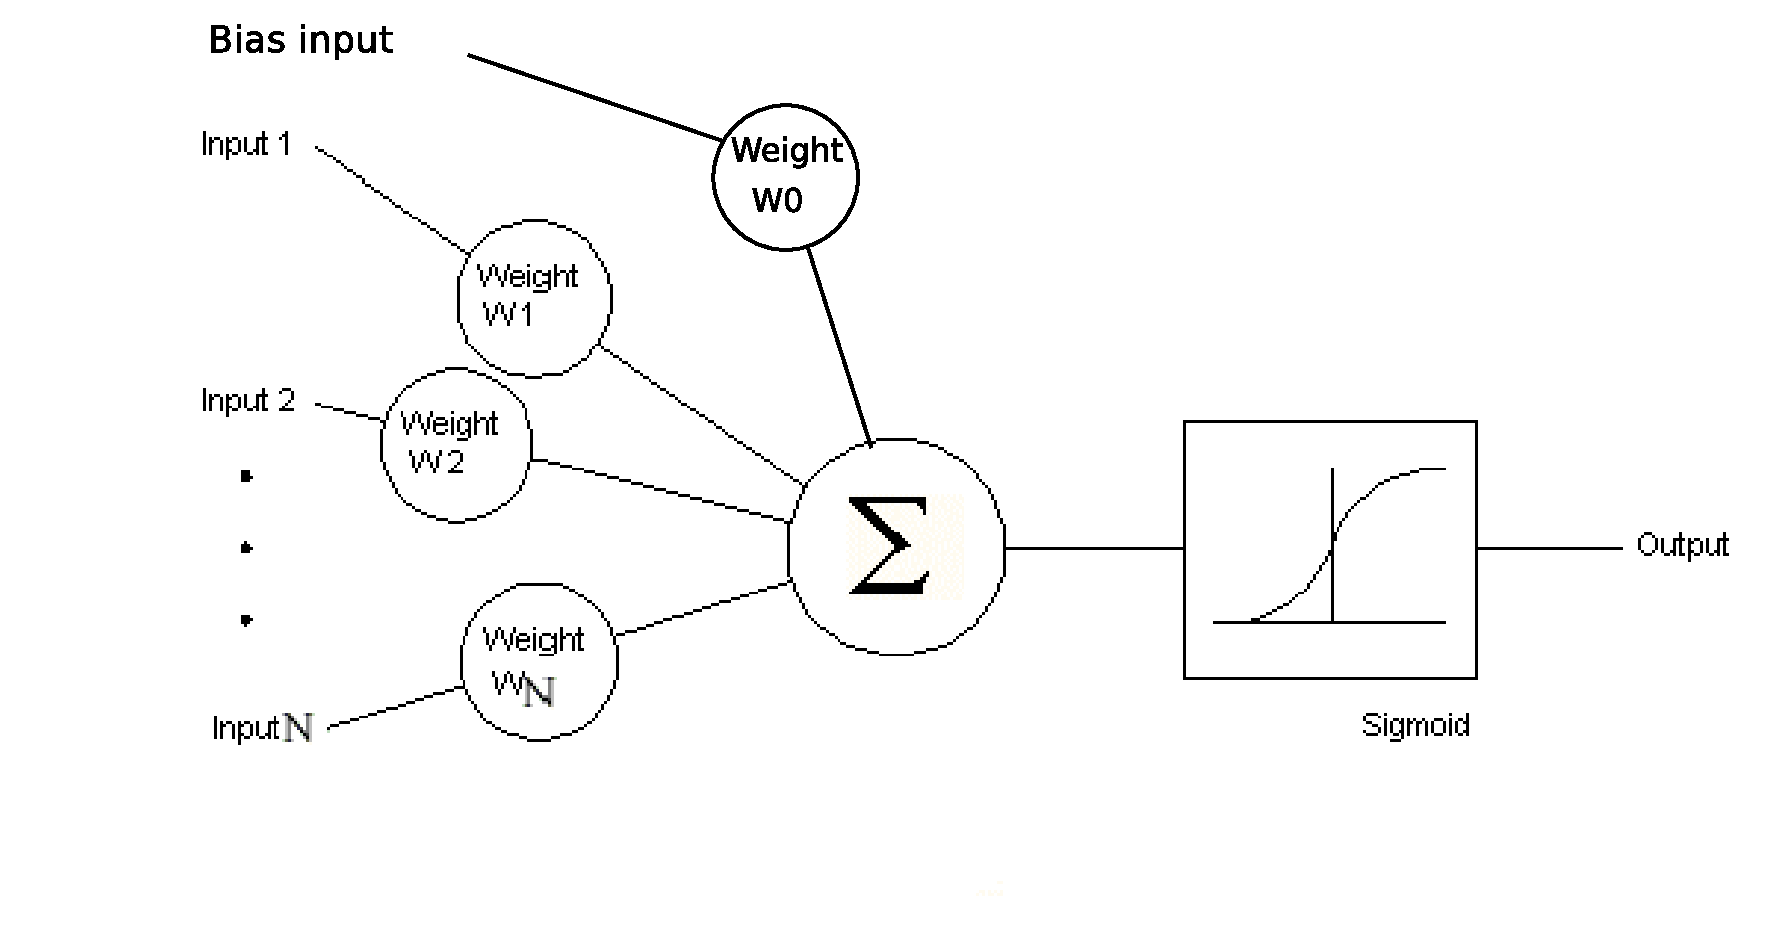
\includegraphics[scale=0.4]{Figures/perceptr.eps}
          \caption{An example of a unit (Sigmoid).}
          \label{fig:unit}
        \end{figure}
   
      \subsection{Computing the output}
        A computational unit in a network has two main components: a \emph{calculation/activation function} and
        an \emph{error function}. The activation function of a unit is the function that the unit applies to the
        sum of all of the inputs multiplied by the weights. Naturally, all of the units that are inputs to a given
        unit $n$ have to have completed their computation before $n$ can proceed. This is no a problem though, as an
        acyclic network implies that a partial ordering of units exist such that the above rule is enforceable. 

        If we view the inputs and weights as vectors $\vec{x}$
        and $\vec{w}$, we can express the output $o$ of a given unit as
        \begin{equation}
           o = f(\vec{w} \cdot \vec{x})
        \end{equation}
        where $f(x)$ is the activation function of the unit.
        There are many different types of activation function and not all of them have been used in this network.
        The ones that have been used are explained in detail below. 
            
      \subsection{Calculating the error}
        The error function of a unit calculates the \emph{training error}. In reality, a given unit has
        two error functions, one if it is an output unit, and another if it hidden. There is also an
        overall error $E$ for the entire network.

        We can picture the \emph{hypothesis space} of a single unit learning a given function by imagining a surface
        in $n$-dimensional space (where $n$ is the number of inputs) plotted as all of the possible values
        for each input weight against $E$. The lowest point on this surface is the global minimum for the unit.
        
        The aim of a network training algorithm is to tune the weights to this global minimum for each unit.
        To achieve this, a greedy method known as \emph{gradient descent} is utilised. Gradient descent is
        an integral part of the backpropagation algorithm and basically calculates the steepest descent of 
        the error surface and updates the weights.
    
        As an example, lets train a linear unit -- which just outputs a linear combination of its inputs --
        with regards to the least mean squares (LMS) error function for the network (which will just be this
        one unit):
        \begin{equation}
          E(\vec{w}) \equiv \frac{1}{2} \sum_{d \in D}(t_d - o_d)^{2}
        \end{equation}       

        where $D$ is the set of training examples and $t_d$ and $o_d$ are the target and actual output values
        for the training example $d$ respectively. As this is a linear unit, we express $E$ as a function of
        the weight vector $\vec{w}$ and we assume that $D$ is fixed through all of the training.

        To get the gradient of the surface so that we can calculate the steepest descent is to find the derivative
        of $E$ with respect to $\vec{w}$. In notation, this is $\nabla E(\vec{w})$ which itself is a vector.
        \begin{equation}
          \nabla E(\vec{w}) \equiv \left\langle  \frac{\partial E}{\partial w_0}, \frac{\partial E}{\partial w_1}, \cdot\cdot\cdot, \frac{\partial E}{\partial w_n} \right\rangle  
        \end{equation}
           
        This vector shows us the direction for the steepest increase in $E$. We want to go the exact opposite way
        from this, so we negate the result. We also multiply this result by a positive constant $\eta$ called the
        \emph{learning rate} which determines the step size in our gradient descent. If $\eta$ is too low, the
        descent will be slow. If it's too high though, the training may not converge to a minimum and may bounce
        around the bottom of the curve. 

        Putting it all together, we see the training rule for gradient descent is:

        \begin{equation}
           \vec{w} \leftarrow \vec{w} + \Delta\vec{w}
        \end{equation}
         
        where

        \begin{equation}
           \Delta\vec{w} = -\eta\nabla E(\vec{w})
        \end{equation} 
        It's clear to see that this method will (provided $\eta$ is small enough) converge to a minimum. 
        But what actually is $\nabla E(\vec{w})$? This can be found by differentiating $E$ for each $w_i$ in $\vec{w}$ :

        \begin{align*} \label{eq:diffme}
           \frac{\partial E}{\partial w_i} &= \frac{\partial}{\partial w_i}  \frac{1}{2} \sum_{d \in D}(t_d - o_d)^{2} \\
           &= \frac{1}{2} \sum_{d \in D} \frac{\partial}{\partial w_i}(t_d - o_d)^{2} \\
           &= \frac{1}{2} \sum_{d \in D}2(t_d - o_d) \frac{\partial}{\partial w_i} (t_d - o_d) \\
           &= \sum_{d \in D}(t_d - o_d)\frac{\partial}{\partial w_i}(t_d - \vec{w} \cdot \vec{x_d}) \\
           \frac{\partial E}{\partial w_i} &= \sum_{d \in D}(t_d - o_d)(-x_{id})
        \end{align*}
 
        Where $x_{id}$ here is the input value $x_i$ for training example $d$. This equation yields the weight
        update rule for an individual weight $w_i$ as:

        \begin{equation}
           w_i \leftarrow w_i + \Delta w_i 
        \end{equation}
        where
         \begin{equation}
           \Delta w_i = \eta \sum_{d \in D}(t_d - o_d)x_{id}
         \end{equation}
      
        

      \subsection{Backpropagation} \label{backprop}
        The above method is suitable only for networks with no hidden layers. To train multilayer networks,
        we have to use an extension of gradient descent: backpropagation.
        Because backpropagation deals with multiple output units, we begin by redefining our $E$ to sum over all
        the network outputs:
        
        \begin{equation}
          E(\vec{w}) \equiv \frac{1}{2} \sum_{d \in D} \sum_{k \in outputs} (t_{kd} - o_{kd})^2  
        \end{equation}   

        Here, $outputs$ is the set of all network output units and $t_{kd}$ and $o_{kd}$ are the target and output
        values associated with the $k^{th}$ output for example $d$. The derivative of this new $E$ is:

        \begin{equation} \label{eq:backdiff}
          \frac{\partial E_d}{\partial w_{ij}}  = - (t_j - o_j)o_j(1 - o_j)x_{ij}
        \end{equation}

        Where $w_{ij}$ and $x_{ij}$ are the weights and inputs from unit $j$ to unit $i$. A full derivation of this
        is available (but not required for understanding this paper) from page 101 onwards in \cite{Mitchell.97}.
        We now have a new delta rule for updating the weights to the output layers:
  
        \begin{equation}
          \Delta w_{ij}  = -\eta\frac{\partial E_d}{\partial w_{ij}} = \eta (t_j - o_j)o_j(1 - o_j)x_{ij}
        \end{equation}

        This is not enough though, we still have to propagate the error back through the hidden layers.
        To do so, we define a new set $Downstream(j)$ which is the set of all units that a given unit $j$ outputs
        to. This is the second error term that a unit can possess and it is defined as:

        \begin{equation} \label{equation:hidden} 
          \delta_j = \frac{df(x)}{dx} \sum_{k \in Downstream(j)} \delta_k w_{kj} 
        \end{equation}  
        where $^{df(x)}/_{dx}$ is the derivative of the activation function of unit $j$ and $\delta_i$ is the
        error term of a given unit $i$.

        The delta in the weight update rule for hidden units is therefore:
        \begin{equation}
          \Delta w_{ji} = \eta \delta_j x_{ji}
        \end{equation}
        
        Obviously, linear units cannot be used as hidden layer units because their activation function is 
        non-differentiable. To counter this, we introduce units that output a continuous function of their
        input, a canonical example of this is the sigmoid $\sigma$ defined as:
        \begin{equation}
          \sigma(x) = \frac{1}{1+e^{a(-x)}}
        \end{equation}
        where $a$ is an offset constant which controls how steep the function is. The derivative, used in equation
        \ref{equation:hidden} can also be easily reduced to $ ^{d\sigma(x)}/_{dx} = \sigma(x) \cdot (1 - \sigma(x))$
        which is a nice and neat expression in terms of its output.

        \subsection{Classification} \label{sec:crosse}
          Currently the primary usage for ANNs is in instance classification. For this, we require a new
          method of working out the error over a given network.
         
          Suppose we have a 2 class dataset, we can build a network with a single output unit which
          calculates the \emph{probability} of class 1 over class 0. We apply a discriminant value 
          $y =0.5$ to determine the resulting class of the input values.
        
          The \emph{cross entropy} of an acyclic classification network is defined as:

          \begin{equation}
            E(\vec{w}) \equiv  - \sum_{d \in D} \sum_{k \in outputs}   t_{kd}\log o_{kd} + (1 - t_{kd})\log(1-o_{kd})  
          \end{equation}
         
          We differentiate as in equation \ref{eq:backdiff} and obtain a rather small result:
 
          \begin{equation}
             \frac{\partial E}{\partial w_{ij}} = -( t_{j} - o_{j} )
          \end{equation} 
           
          So that our new update rule for classification outputs is:

          \begin{equation}
             \Delta w_{ji} =  \eta (t_{j} - o_{j})  
          \end{equation}

      All of the trained networks use these to calculate the classification error and adjust the weights
      whilst training.
 
%%%%%%%%%%%%%%%%%%%%%%%%%%%%%%%%%%%%%%%%%%%%%%%%%%%%%%%%%%%%%%%%%%%%%%%%%%%%%%%%%%%%%%%%%%%%%%%%%%%%%%%%%%%%%%%%%%%%%%% 
%%%%%%%%%%%%%%%%%%%%%%%%%%%%%%%%%%%%%%%%%%% APPENDIX C %%%%%%%%%%%%%%%%%%%%%%%%%%%%%%%%%%%%%%%%%%%%%%%%%%%%%%%%%%%%%%%%
%%%%%%%%%%%%%%%%%%%%%%%%%%%%%%%%%%%%%%%%%%%%%%%%%%%%%%%%%%%%%%%%%%%%%%%%%%%%%%%%%%%%%%%%%%%%%%%%%%%%%%%%%%%%%%%%%%%%%%%
  \section{The PCP theorem} \label{sec:PCP}
    The \emph{Probabilistically checkable proofs} (PCP) theorem is one of the most important theorems
    in the field of hardness of approximation. It states that every problem contained in the complexity class
    NP has at least one probabilistically checkable proof with a constant \emph{query complexity}\footnote{We can view
    query complexity using the decision tree model introduced in section \ref{sec:NPint}. The query complexity of
    of such a tree is the maximum possible depth that this decision tree can reach.} and logarithmic
    randomness. 

    We consider probabilistically checkable proofs in the context of a prover $P$ which writes a proof
    and a verifier $V$ which checks it with the following properties:
    \begin{itemize*}
      \item Completeness. $\forall x \in L$, $P$ can write a proof of length $poly(|x|)$ that $V$ accepts.  
      \item Soundness. $\forall x \notin L$, No matter which $poly(|x|)$ proof $P$ writes, $V$ rejects with
            a probability of $1/2$.
    \end{itemize*}
    A probabilistically checkable proof $x \in L \subset NP$ is one that $P$ can write a proof of $poly(|x|)$
    bits for, then presents this proof to   
    $V$ which performs some deterministic computation and then uses $\log(|x|)$ bits of randomness
    to select $T$ random locations in the proof. Here $T$ is a
    universal constant; say, 100. $V$ also uses the random bits to produce a deterministic test $\theta$ on
    $T$ bits. 
    $V$ reads the bits in the $T$ random locations, performs its test $\theta$ on them and then accepts or rejects
    \cite{PCPLec}.
    
    Note here that, while $V$ can accepts false proofs with a probability of 1/2, we can manage this probability
    through repetition. If we were to repeat the process $n$ times, we will read in $nT$ bits and accept false
    proofs with a probability of at most $2^{-n}$.

    This dissertation won't go into the proof of the PCP theorem as it is\ldots rather involved. An interested
    reader can read the separately produced original papers \cite{PCP1}\cite{PCP2} or read Irit Dinur's 2005 alternate,
    much shorter proof 
    \cite{PCP3}.

    The history of the PCP theorem is a long and quite interesting one that started with the
    investigation into interactive proof systems (IP) and a short summary can be read here
    \url{http://people.csail.mit.edu/dmoshkov/courses/pcp/pcp-history.pdf}. 

    As a result of the PCP theorem, we can characterise the classes of NP by their randomness complexity and
    query complexity -- PCP[$r(n)$, $q(n)$]:

    \begin{itemize*}
      \item NP = PCP[$O(log n)$, $O(1)$]
      \item P = PCP[0,0] -- there is no randomness and no access to a proof. \\
            \emph{Or} PCP[$O(log n)$, 0] -- logarithmic randomness doesn't help a deterministic machine as it can easily try
            all random strings of polynomial length in polynomial time. \\
            \emph{Or} PCP[0, $O(log n)$] -- without randomness, we can see the proof as a fixed logarithmic sized string.
            It can easily try all possible logarithmic sized proofs in polynomial time.  
    \end{itemize*} 
    
    For the NP case, we only need $log(n)$ bits of randomness and the entire proof to verify it in polynomial time.
    For the P cases, it's clear to see that all 3 cases presented are equivalent as it doesn't matter what randomness
    introduced because we can check the whole proof in polynomial time anyway!

    In any case, the main message is that: All problems in NP can have a proof of length $poly(|x|)$ written about
    them, and this proof can be checked in polynomial time by a verifier using $\log(|x|)$ bits of randomness to
    check $C$ locations in the proof and will always return `true' if the proof is correct, and will reject an 
    incorrect proof 1/2 of the time.  
    

%%%%%%%%%%%%%%%%%%%%%%%%%%%%%%%%%%%%%%%%%%%%%%%%%%%%%%%%%%%%%%%%%%%%%%%%%%%%%%%%%%%%%%%%%%%%%%%%%%%%%%%%%%%%%%%%%%%%%%% 
%%%%%%%%%%%%%%%%%%%%%%%%%%%%%%%%%%%%%%%%%%% APPENDIX D %%%%%%%%%%%%%%%%%%%%%%%%%%%%%%%%%%%%%%%%%%%%%%%%%%%%%%%%%%%%%%%%
%%%%%%%%%%%%%%%%%%%%%%%%%%%%%%%%%%%%%%%%%%%%%%%%%%%%%%%%%%%%%%%%%%%%%%%%%%%%%%%%%%%%%%%%%%%%%%%%%%%%%%%%%%%%%%%%%%%%%%%

  \section{Dataset plots} \label{app:DS}   

   \begin{figure}[H] 
     \centering
     \includegraphics[scale=0.8]{Figures/PResults60-0.2.ps}
     \caption{Plot of accuracy against p value for $\alpha = 0.2$.}
     \label{fig:0.2}  
   \end{figure}

   \begin{figure}[H]
     \centering
     \includegraphics[scale=0.8]{Figures/PResults60-0.3.ps}
     \caption{Plots of accuracy against p value for $\alpha = 0.3$.}
     \label{fig:0.3} 
   \end{figure}

   \begin{figure}[H]
     \centering
     \includegraphics[scale=0.8]{Figures/PResults60-0.4.ps}
     \caption{Plot of accuracy against p value for $\alpha = 0.4$.}
     \label{fig:0.4}
   \end{figure}

   \begin{figure}[H]
     \centering
     \includegraphics[scale=0.8]{Figures/PResults60-0.5.ps}
     \caption{Plots of accuracy against p value for $\alpha = 0.5$.}
     \label{fig:0.5}
   \end{figure}

   \begin{figure}[H]
     \centering
     \includegraphics[scale=0.8]{Figures/PResults60-0.6.ps}
     \caption{Plot of accuracy against p value for $\alpha = 0.6$.}
     \label{fig:0.6}
   \end{figure}

   \begin{figure}[H]
     \centering
     \includegraphics[scale=0.8]{Figures/PResults60-0.7.ps}
     \caption{Plots of accuracy against p value for $\alpha = 0.7$.}
     \label{fig:0.7}
   \end{figure}

   \begin{figure}[H]
     \centering
     \includegraphics[scale=0.8]{Figures/PResults60-0.8.ps}
     \caption{Plot of accuracy against p value for $\alpha = 0.8$.}
     \label{fig:0.8}
   \end{figure}

   \begin{figure}[H]
     \centering
     \includegraphics[scale=0.8]{Figures/PResults60-0.9.ps}
     \caption{Plots of accuracy against p value for $\alpha = 0.9$.}
     \label{fig:0.9}
   \end{figure}

%%%%%%%%%%%%%%%%%%%%%%%%%%%%%%%%%%%%%%%%%%%%%%%%%%%%%%%%%%%%%%%%%%%%%%%%%%%%%%%%%%%%%%%%%%%%%%%%%%%%%%%%%%%%%%%%%%%%%%%
%%%%%%%%%%%%%%%%%%%%%%%%%%%%%%%%%%%%% THE SECRET APPENDIX!! %%%%%%%%%%%%%%%%%%%%%%%%%%%%%%%%%%%%%%%%%%%%%%%%%%%%%%%%%%
%%%%%%%%%%%%%%%%%%%%%%%%%%%%%%%%%%%%%%%%%%%%%%%%%%%%%%%%%%%%%%%%%%%%%%%%%%%%%%%%%%%%%%%%%%%%%%%%%%%%%%%%%%%%%%%%%%%%%%%

% \section{Code} \label{code}
%  This appendix is a listing of all the code used in this dissertation\ldots It's quite long\ldots
%  
%   \subsection{The graph}
%     This is the listing for the Graph data structure featured in section \ref{sec:theGraph}.
%     It is used by almost all of the dissertation functions.
     
%     \subsubsection{Graph class}
%       \lstinputlisting{/u1/cs4/jrd5/Dissertation/Code/Graph/Graph.java}  

%     \subsubsection{Edge class}
%       \lstinputlisting{/u1/cs4/jrd5/Dissertation/Code/Graph/Edge.java}

%     \subsubsection{Vertex class}
%       \lstinputlisting{/u1/cs4/jrd5/Dissertation/Code/Graph/Vertex.java}

%   \subsection{The vertex cover functions}
%     This is the listing for the greedy vertex covering algorithms as discussed in section \ref{sec:GREEDY}.
%     The algorithms are labeled here 1 -- 4 as they were in the section. These are tied together by a driver
%     class that instantiates everything and actually runs the program. 

%     \subsubsection{Driver class}
%        \lstinputlisting{/u1/cs4/jrd5/Dissertation/Code/VCPNew/Driver.java}

%     \subsubsection{Algorithm 1}
%        \lstinputlisting{/u1/cs4/jrd5/Dissertation/Code/VCPNew/Algorithms/VertexCover1.java}

%     \subsubsection{Algorithm 2}

%     \subsubsection{Algorithm 3}
 
%     \subsubsection{Algorithm 4}       

  \bibliographystyle{alpha}
  \bibliography{citation}

\end{document}
